\documentclass[twoside]{book}

% Packages required by doxygen
\usepackage{fixltx2e}
\usepackage{calc}
\usepackage{doxygen}
\usepackage[export]{adjustbox} % also loads graphicx
\usepackage{graphicx}
\usepackage[utf8]{inputenc}
\usepackage{makeidx}
\usepackage{multicol}
\usepackage{multirow}
\PassOptionsToPackage{warn}{textcomp}
\usepackage{textcomp}
\usepackage[nointegrals]{wasysym}
\usepackage[table]{xcolor}

% Font selection
\usepackage[T1]{fontenc}
\usepackage[scaled=.90]{helvet}
\usepackage{courier}
\usepackage{amssymb}
\usepackage{sectsty}
\renewcommand{\familydefault}{\sfdefault}
\allsectionsfont{%
  \fontseries{bc}\selectfont%
  \color{darkgray}%
}
\renewcommand{\DoxyLabelFont}{%
  \fontseries{bc}\selectfont%
  \color{darkgray}%
}
\newcommand{\+}{\discretionary{\mbox{\scriptsize$\hookleftarrow$}}{}{}}

% Page & text layout
\usepackage{geometry}
\geometry{%
  a4paper,%
  top=2.5cm,%
  bottom=2.5cm,%
  left=2.5cm,%
  right=2.5cm%
}
\tolerance=750
\hfuzz=15pt
\hbadness=750
\setlength{\emergencystretch}{15pt}
\setlength{\parindent}{0cm}
\setlength{\parskip}{3ex plus 2ex minus 2ex}
\makeatletter
\renewcommand{\paragraph}{%
  \@startsection{paragraph}{4}{0ex}{-1.0ex}{1.0ex}{%
    \normalfont\normalsize\bfseries\SS@parafont%
  }%
}
\renewcommand{\subparagraph}{%
  \@startsection{subparagraph}{5}{0ex}{-1.0ex}{1.0ex}{%
    \normalfont\normalsize\bfseries\SS@subparafont%
  }%
}
\makeatother

% Headers & footers
\usepackage{fancyhdr}
\pagestyle{fancyplain}
\fancyhead[LE]{\fancyplain{}{\bfseries\thepage}}
\fancyhead[CE]{\fancyplain{}{}}
\fancyhead[RE]{\fancyplain{}{\bfseries\leftmark}}
\fancyhead[LO]{\fancyplain{}{\bfseries\rightmark}}
\fancyhead[CO]{\fancyplain{}{}}
\fancyhead[RO]{\fancyplain{}{\bfseries\thepage}}
\fancyfoot[LE]{\fancyplain{}{}}
\fancyfoot[CE]{\fancyplain{}{}}
\fancyfoot[RE]{\fancyplain{}{\bfseries\scriptsize Generated by Doxygen }}
\fancyfoot[LO]{\fancyplain{}{\bfseries\scriptsize Generated by Doxygen }}
\fancyfoot[CO]{\fancyplain{}{}}
\fancyfoot[RO]{\fancyplain{}{}}
\renewcommand{\footrulewidth}{0.4pt}
\renewcommand{\chaptermark}[1]{%
  \markboth{#1}{}%
}
\renewcommand{\sectionmark}[1]{%
  \markright{\thesection\ #1}%
}

% Indices & bibliography
\usepackage{natbib}
\usepackage[titles]{tocloft}
\setcounter{tocdepth}{3}
\setcounter{secnumdepth}{5}
\makeindex

% Hyperlinks (required, but should be loaded last)
\usepackage{ifpdf}
\ifpdf
  \usepackage[pdftex,pagebackref=true]{hyperref}
\else
  \usepackage[ps2pdf,pagebackref=true]{hyperref}
\fi
\hypersetup{%
  colorlinks=true,%
  linkcolor=blue,%
  citecolor=blue,%
  unicode%
}

% Custom commands
\newcommand{\clearemptydoublepage}{%
  \newpage{\pagestyle{empty}\cleardoublepage}%
}

\usepackage{caption}
\captionsetup{labelsep=space,justification=centering,font={bf},singlelinecheck=off,skip=4pt,position=top}

%===== C O N T E N T S =====

\begin{document}

% Titlepage & ToC
\hypersetup{pageanchor=false,
             bookmarksnumbered=true,
             pdfencoding=unicode
            }
\pagenumbering{alph}
\begin{titlepage}
\vspace*{7cm}
\begin{center}%
{\Large Autosonography \\[1ex]\large 1 }\\
\vspace*{1cm}
{\large Generated by Doxygen 1.8.12}\\
\end{center}
\end{titlepage}
\clearemptydoublepage
\pagenumbering{roman}
\tableofcontents
\clearemptydoublepage
\pagenumbering{arabic}
\hypersetup{pageanchor=true}

%--- Begin generated contents ---
\chapter{Namespace Index}
\section{Packages}
Here are the packages with brief descriptions (if available)\+:\begin{DoxyCompactList}
\item\contentsline{section}{\hyperlink{namespace_auto_sonography_w_p_f}{Auto\+Sonography\+W\+PF} }{\pageref{namespace_auto_sonography_w_p_f}}{}
\item\contentsline{section}{\hyperlink{namespace_auto_sonography_w_p_f_1_1_properties}{Auto\+Sonography\+W\+P\+F.\+Properties} }{\pageref{namespace_auto_sonography_w_p_f_1_1_properties}}{}
\item\contentsline{section}{\hyperlink{namespace_computer_vision_library}{Computer\+Vision\+Library} \\*Mostly made by Microsoft, based on their Kinect Fusion Explorer which showcases most features of the Kinect A\+PI and Fusion library \href{https://msdn.microsoft.com/en-us/library/dn193975.aspx}{\tt https\+://msdn.\+microsoft.\+com/en-\/us/library/dn193975.\+aspx} }{\pageref{namespace_computer_vision_library}}{}
\item\contentsline{section}{\hyperlink{namespace_robo_library}{Robo\+Library} }{\pageref{namespace_robo_library}}{}
\item\contentsline{section}{\hyperlink{namespace_robo_library_1_1_dummies}{Robo\+Library.\+Dummies} }{\pageref{namespace_robo_library_1_1_dummies}}{}
\item\contentsline{section}{\hyperlink{namespace_robo_library_1_1_interfaces}{Robo\+Library.\+Interfaces} }{\pageref{namespace_robo_library_1_1_interfaces}}{}
\item\contentsline{section}{\hyperlink{namespace_robo_library_1_1_testing_extensions}{Robo\+Library.\+Testing\+Extensions} }{\pageref{namespace_robo_library_1_1_testing_extensions}}{}
\item\contentsline{section}{\hyperlink{namespace_unit_test_computer_vision_library}{Unit\+Test\+Computer\+Vision\+Library} }{\pageref{namespace_unit_test_computer_vision_library}}{}
\item\contentsline{section}{\hyperlink{namespace_unit_test_robot_library}{Unit\+Test\+Robot\+Library} }{\pageref{namespace_unit_test_robot_library}}{}
\end{DoxyCompactList}

\chapter{Hierarchical Index}
\section{Class Hierarchy}
This inheritance list is sorted roughly, but not completely, alphabetically\+:\begin{DoxyCompactList}
\item Application\begin{DoxyCompactList}
\item \contentsline{section}{Auto\+Sonography\+W\+P\+F.\+App}{\pageref{class_auto_sonography_w_p_f_1_1_app}}{}
\item \contentsline{section}{Auto\+Sonography\+W\+P\+F.\+App}{\pageref{class_auto_sonography_w_p_f_1_1_app}}{}
\item \contentsline{section}{Auto\+Sonography\+W\+P\+F.\+App}{\pageref{class_auto_sonography_w_p_f_1_1_app}}{}
\item \contentsline{section}{Auto\+Sonography\+W\+P\+F.\+App}{\pageref{class_auto_sonography_w_p_f_1_1_app}}{}
\item \contentsline{section}{Auto\+Sonography\+W\+P\+F.\+App}{\pageref{class_auto_sonography_w_p_f_1_1_app}}{}
\end{DoxyCompactList}
\item \contentsline{section}{Robo\+Library.\+Camera\+To\+Robot\+Calibrator}{\pageref{class_robo_library_1_1_camera_to_robot_calibrator}}{}
\item \contentsline{section}{Computer\+Vision\+Library.\+Color\+Vertex\+Slicer}{\pageref{class_computer_vision_library_1_1_color_vertex_slicer}}{}
\item \contentsline{section}{Computer\+Vision\+Library.\+Computer\+Vision\+Master}{\pageref{class_computer_vision_library_1_1_computer_vision_master}}{}
\item \contentsline{section}{Robo\+Library.\+Data}{\pageref{class_robo_library_1_1_data}}{}
\item \contentsline{section}{Robo\+Library.\+Dummies.\+Dummy\+U\+R10}{\pageref{class_robo_library_1_1_dummies_1_1_dummy_u_r10}}{}
\item \contentsline{section}{Robo\+Library.\+Interfaces.\+I\+Analyzer}{\pageref{interface_robo_library_1_1_interfaces_1_1_i_analyzer}}{}
\begin{DoxyCompactList}
\item \contentsline{section}{Robo\+Library.\+Analyzer}{\pageref{class_robo_library_1_1_analyzer}}{}
\end{DoxyCompactList}
\item I\+Component\+Connector\begin{DoxyCompactList}
\item \contentsline{section}{Auto\+Sonography\+W\+P\+F.\+\_\+3\+D\+Scan\+Menu}{\pageref{class_auto_sonography_w_p_f_1_1__3_d_scan_menu}}{}
\item \contentsline{section}{Auto\+Sonography\+W\+P\+F.\+\_\+3\+D\+Scan\+Menu}{\pageref{class_auto_sonography_w_p_f_1_1__3_d_scan_menu}}{}
\item \contentsline{section}{Auto\+Sonography\+W\+P\+F.\+\_\+3\+D\+Scan\+Menu}{\pageref{class_auto_sonography_w_p_f_1_1__3_d_scan_menu}}{}
\item \contentsline{section}{Auto\+Sonography\+W\+P\+F.\+\_\+3\+D\+Scan\+Menu}{\pageref{class_auto_sonography_w_p_f_1_1__3_d_scan_menu}}{}
\item \contentsline{section}{Auto\+Sonography\+W\+P\+F.\+Main\+Window}{\pageref{class_auto_sonography_w_p_f_1_1_main_window}}{}
\item \contentsline{section}{Auto\+Sonography\+W\+P\+F.\+Main\+Window}{\pageref{class_auto_sonography_w_p_f_1_1_main_window}}{}
\item \contentsline{section}{Auto\+Sonography\+W\+P\+F.\+Main\+Window}{\pageref{class_auto_sonography_w_p_f_1_1_main_window}}{}
\item \contentsline{section}{Auto\+Sonography\+W\+P\+F.\+Main\+Window}{\pageref{class_auto_sonography_w_p_f_1_1_main_window}}{}
\item \contentsline{section}{Auto\+Sonography\+W\+P\+F.\+Main\+Window}{\pageref{class_auto_sonography_w_p_f_1_1_main_window}}{}
\item \contentsline{section}{Auto\+Sonography\+W\+P\+F.\+Main\+Window}{\pageref{class_auto_sonography_w_p_f_1_1_main_window}}{}
\item \contentsline{section}{Auto\+Sonography\+W\+P\+F.\+Ultrasound\+Scan\+Menu}{\pageref{class_auto_sonography_w_p_f_1_1_ultrasound_scan_menu}}{}
\item \contentsline{section}{Auto\+Sonography\+W\+P\+F.\+Ultrasound\+Scan\+Menu}{\pageref{class_auto_sonography_w_p_f_1_1_ultrasound_scan_menu}}{}
\item \contentsline{section}{Auto\+Sonography\+W\+P\+F.\+Ultrasound\+Scan\+Menu}{\pageref{class_auto_sonography_w_p_f_1_1_ultrasound_scan_menu}}{}
\item \contentsline{section}{Auto\+Sonography\+W\+P\+F.\+Ultrasound\+Scan\+Menu}{\pageref{class_auto_sonography_w_p_f_1_1_ultrasound_scan_menu}}{}
\end{DoxyCompactList}
\item \contentsline{section}{Robo\+Library.\+Interfaces.\+I\+Reader}{\pageref{interface_robo_library_1_1_interfaces_1_1_i_reader}}{}
\begin{DoxyCompactList}
\item \contentsline{section}{Robo\+Library.\+Dummies.\+Dummy\+Reader}{\pageref{class_robo_library_1_1_dummies_1_1_dummy_reader}}{}
\item \contentsline{section}{Robo\+Library.\+Reader}{\pageref{class_robo_library_1_1_reader}}{}
\end{DoxyCompactList}
\item \contentsline{section}{Robo\+Library.\+Interfaces.\+I\+Writer}{\pageref{interface_robo_library_1_1_interfaces_1_1_i_writer}}{}
\begin{DoxyCompactList}
\item \contentsline{section}{Robo\+Library.\+Dummies.\+Dummy\+Writer}{\pageref{class_robo_library_1_1_dummies_1_1_dummy_writer}}{}
\item \contentsline{section}{Robo\+Library.\+Writer}{\pageref{class_robo_library_1_1_writer}}{}
\end{DoxyCompactList}
\item \contentsline{section}{Computer\+Vision\+Library.\+Kinect\+Fusionizer}{\pageref{class_computer_vision_library_1_1_kinect_fusionizer}}{}
\item \contentsline{section}{Robo\+Library.\+Logic}{\pageref{class_robo_library_1_1_logic}}{}
\item \contentsline{section}{Computer\+Vision\+Library.\+Mesh}{\pageref{class_computer_vision_library_1_1_mesh}}{}
\item \contentsline{section}{Robo\+Library.\+Mod\+Bus}{\pageref{class_robo_library_1_1_mod_bus}}{}
\item \contentsline{section}{Robo\+Library.\+Path\+Creator}{\pageref{class_robo_library_1_1_path_creator}}{}
\item \contentsline{section}{Robo\+Library.\+Path\+Feeder}{\pageref{class_robo_library_1_1_path_feeder}}{}
\item \contentsline{section}{Computer\+Vision\+Library.\+P\+L\+Y\+Exporter}{\pageref{class_computer_vision_library_1_1_p_l_y_exporter}}{}
\item \contentsline{section}{Robo\+Library.\+Robo\+Master}{\pageref{class_robo_library_1_1_robo_master}}{}
\item \contentsline{section}{Robo\+Library.\+Testing\+Extensions.\+Shape\+Generator}{\pageref{class_robo_library_1_1_testing_extensions_1_1_shape_generator}}{}
\item \contentsline{section}{Robo\+Library.\+U\+R\+Pose}{\pageref{class_robo_library_1_1_u_r_pose}}{}
\item \contentsline{section}{Unit\+Test\+Computer\+Vision\+Library.\+U\+T\+Color\+Vertex\+Slicer}{\pageref{class_unit_test_computer_vision_library_1_1_u_t_color_vertex_slicer}}{}
\item \contentsline{section}{Unit\+Test\+Robot\+Library.\+U\+T\+Path\+Feeder}{\pageref{class_unit_test_robot_library_1_1_u_t_path_feeder}}{}
\item Window\begin{DoxyCompactList}
\item \contentsline{section}{Auto\+Sonography\+W\+P\+F.\+\_\+3\+D\+Scan\+Menu}{\pageref{class_auto_sonography_w_p_f_1_1__3_d_scan_menu}}{}
\item \contentsline{section}{Auto\+Sonography\+W\+P\+F.\+\_\+3\+D\+Scan\+Menu}{\pageref{class_auto_sonography_w_p_f_1_1__3_d_scan_menu}}{}
\item \contentsline{section}{Auto\+Sonography\+W\+P\+F.\+\_\+3\+D\+Scan\+Menu}{\pageref{class_auto_sonography_w_p_f_1_1__3_d_scan_menu}}{}
\item \contentsline{section}{Auto\+Sonography\+W\+P\+F.\+\_\+3\+D\+Scan\+Menu}{\pageref{class_auto_sonography_w_p_f_1_1__3_d_scan_menu}}{}
\item \contentsline{section}{Auto\+Sonography\+W\+P\+F.\+\_\+3\+D\+Scan\+Menu}{\pageref{class_auto_sonography_w_p_f_1_1__3_d_scan_menu}}{}
\item \contentsline{section}{Auto\+Sonography\+W\+P\+F.\+Main\+Window}{\pageref{class_auto_sonography_w_p_f_1_1_main_window}}{}
\item \contentsline{section}{Auto\+Sonography\+W\+P\+F.\+Main\+Window}{\pageref{class_auto_sonography_w_p_f_1_1_main_window}}{}
\item \contentsline{section}{Auto\+Sonography\+W\+P\+F.\+Main\+Window}{\pageref{class_auto_sonography_w_p_f_1_1_main_window}}{}
\item \contentsline{section}{Auto\+Sonography\+W\+P\+F.\+Main\+Window}{\pageref{class_auto_sonography_w_p_f_1_1_main_window}}{}
\item \contentsline{section}{Auto\+Sonography\+W\+P\+F.\+Main\+Window}{\pageref{class_auto_sonography_w_p_f_1_1_main_window}}{}
\item \contentsline{section}{Auto\+Sonography\+W\+P\+F.\+Main\+Window}{\pageref{class_auto_sonography_w_p_f_1_1_main_window}}{}
\item \contentsline{section}{Auto\+Sonography\+W\+P\+F.\+Main\+Window}{\pageref{class_auto_sonography_w_p_f_1_1_main_window}}{}
\item \contentsline{section}{Auto\+Sonography\+W\+P\+F.\+Ultrasound\+Scan\+Menu}{\pageref{class_auto_sonography_w_p_f_1_1_ultrasound_scan_menu}}{}
\item \contentsline{section}{Auto\+Sonography\+W\+P\+F.\+Ultrasound\+Scan\+Menu}{\pageref{class_auto_sonography_w_p_f_1_1_ultrasound_scan_menu}}{}
\item \contentsline{section}{Auto\+Sonography\+W\+P\+F.\+Ultrasound\+Scan\+Menu}{\pageref{class_auto_sonography_w_p_f_1_1_ultrasound_scan_menu}}{}
\item \contentsline{section}{Auto\+Sonography\+W\+P\+F.\+Ultrasound\+Scan\+Menu}{\pageref{class_auto_sonography_w_p_f_1_1_ultrasound_scan_menu}}{}
\item \contentsline{section}{Auto\+Sonography\+W\+P\+F.\+Ultrasound\+Scan\+Menu}{\pageref{class_auto_sonography_w_p_f_1_1_ultrasound_scan_menu}}{}
\end{DoxyCompactList}
\end{DoxyCompactList}

\chapter{Class Index}
\section{Class List}
Here are the classes, structs, unions and interfaces with brief descriptions\+:\begin{DoxyCompactList}
\item\contentsline{section}{\hyperlink{class_auto_sonography_w_p_f_1_1__3_d_scan_menu}{Auto\+Sonography\+W\+P\+F.\+\_\+3\+D\+Scan\+Menu} \\*Interaction logic for \+\_\+3\+D\+Scan\+Menu.\+xaml }{\pageref{class_auto_sonography_w_p_f_1_1__3_d_scan_menu}}{}
\item\contentsline{section}{\hyperlink{class_robo_library_1_1_analyzer}{Robo\+Library.\+Analyzer} }{\pageref{class_robo_library_1_1_analyzer}}{}
\item\contentsline{section}{\hyperlink{class_auto_sonography_w_p_f_1_1_app}{Auto\+Sonography\+W\+P\+F.\+App} \\*Interaction logic for App.\+xaml }{\pageref{class_auto_sonography_w_p_f_1_1_app}}{}
\item\contentsline{section}{\hyperlink{class_robo_library_1_1_camera_to_robot_calibrator}{Robo\+Library.\+Camera\+To\+Robot\+Calibrator} }{\pageref{class_robo_library_1_1_camera_to_robot_calibrator}}{}
\item\contentsline{section}{\hyperlink{class_computer_vision_library_1_1_color_vertex_slicer}{Computer\+Vision\+Library.\+Color\+Vertex\+Slicer} }{\pageref{class_computer_vision_library_1_1_color_vertex_slicer}}{}
\item\contentsline{section}{\hyperlink{class_computer_vision_library_1_1_computer_vision_master}{Computer\+Vision\+Library.\+Computer\+Vision\+Master} }{\pageref{class_computer_vision_library_1_1_computer_vision_master}}{}
\item\contentsline{section}{\hyperlink{class_robo_library_1_1_data}{Robo\+Library.\+Data} }{\pageref{class_robo_library_1_1_data}}{}
\item\contentsline{section}{\hyperlink{class_robo_library_1_1_dummies_1_1_dummy_reader}{Robo\+Library.\+Dummies.\+Dummy\+Reader} }{\pageref{class_robo_library_1_1_dummies_1_1_dummy_reader}}{}
\item\contentsline{section}{\hyperlink{class_robo_library_1_1_dummies_1_1_dummy_u_r10}{Robo\+Library.\+Dummies.\+Dummy\+U\+R10} }{\pageref{class_robo_library_1_1_dummies_1_1_dummy_u_r10}}{}
\item\contentsline{section}{\hyperlink{class_robo_library_1_1_dummies_1_1_dummy_writer}{Robo\+Library.\+Dummies.\+Dummy\+Writer} }{\pageref{class_robo_library_1_1_dummies_1_1_dummy_writer}}{}
\item\contentsline{section}{\hyperlink{interface_robo_library_1_1_interfaces_1_1_i_analyzer}{Robo\+Library.\+Interfaces.\+I\+Analyzer} }{\pageref{interface_robo_library_1_1_interfaces_1_1_i_analyzer}}{}
\item\contentsline{section}{\hyperlink{interface_robo_library_1_1_interfaces_1_1_i_reader}{Robo\+Library.\+Interfaces.\+I\+Reader} }{\pageref{interface_robo_library_1_1_interfaces_1_1_i_reader}}{}
\item\contentsline{section}{\hyperlink{interface_robo_library_1_1_interfaces_1_1_i_writer}{Robo\+Library.\+Interfaces.\+I\+Writer} }{\pageref{interface_robo_library_1_1_interfaces_1_1_i_writer}}{}
\item\contentsline{section}{\hyperlink{class_computer_vision_library_1_1_kinect_fusionizer}{Computer\+Vision\+Library.\+Kinect\+Fusionizer} }{\pageref{class_computer_vision_library_1_1_kinect_fusionizer}}{}
\item\contentsline{section}{\hyperlink{class_robo_library_1_1_logic}{Robo\+Library.\+Logic} }{\pageref{class_robo_library_1_1_logic}}{}
\item\contentsline{section}{\hyperlink{class_auto_sonography_w_p_f_1_1_main_window}{Auto\+Sonography\+W\+P\+F.\+Main\+Window} \\*Interaction logic for Main\+Window.\+xaml }{\pageref{class_auto_sonography_w_p_f_1_1_main_window}}{}
\item\contentsline{section}{\hyperlink{class_computer_vision_library_1_1_mesh}{Computer\+Vision\+Library.\+Mesh} }{\pageref{class_computer_vision_library_1_1_mesh}}{}
\item\contentsline{section}{\hyperlink{class_robo_library_1_1_mod_bus}{Robo\+Library.\+Mod\+Bus} \\*Modbus T\+CP common driver class. This class implements a modbus T\+CP master driver. It supports the following commands\+: }{\pageref{class_robo_library_1_1_mod_bus}}{}
\item\contentsline{section}{\hyperlink{class_robo_library_1_1_path_creator}{Robo\+Library.\+Path\+Creator} }{\pageref{class_robo_library_1_1_path_creator}}{}
\item\contentsline{section}{\hyperlink{class_robo_library_1_1_path_feeder}{Robo\+Library.\+Path\+Feeder} }{\pageref{class_robo_library_1_1_path_feeder}}{}
\item\contentsline{section}{\hyperlink{class_computer_vision_library_1_1_p_l_y_exporter}{Computer\+Vision\+Library.\+P\+L\+Y\+Exporter} }{\pageref{class_computer_vision_library_1_1_p_l_y_exporter}}{}
\item\contentsline{section}{\hyperlink{class_robo_library_1_1_reader}{Robo\+Library.\+Reader} }{\pageref{class_robo_library_1_1_reader}}{}
\item\contentsline{section}{\hyperlink{class_robo_library_1_1_robo_master}{Robo\+Library.\+Robo\+Master} }{\pageref{class_robo_library_1_1_robo_master}}{}
\item\contentsline{section}{\hyperlink{class_robo_library_1_1_testing_extensions_1_1_shape_generator}{Robo\+Library.\+Testing\+Extensions.\+Shape\+Generator} }{\pageref{class_robo_library_1_1_testing_extensions_1_1_shape_generator}}{}
\item\contentsline{section}{\hyperlink{class_auto_sonography_w_p_f_1_1_ultrasound_scan_menu}{Auto\+Sonography\+W\+P\+F.\+Ultrasound\+Scan\+Menu} \\*\hyperlink{class_auto_sonography_w_p_f_1_1_ultrasound_scan_menu}{Ultrasound\+Scan\+Menu} }{\pageref{class_auto_sonography_w_p_f_1_1_ultrasound_scan_menu}}{}
\item\contentsline{section}{\hyperlink{class_robo_library_1_1_u_r_pose}{Robo\+Library.\+U\+R\+Pose} }{\pageref{class_robo_library_1_1_u_r_pose}}{}
\item\contentsline{section}{\hyperlink{class_unit_test_computer_vision_library_1_1_u_t_color_vertex_slicer}{Unit\+Test\+Computer\+Vision\+Library.\+U\+T\+Color\+Vertex\+Slicer} }{\pageref{class_unit_test_computer_vision_library_1_1_u_t_color_vertex_slicer}}{}
\item\contentsline{section}{\hyperlink{class_unit_test_robot_library_1_1_u_t_path_feeder}{Unit\+Test\+Robot\+Library.\+U\+T\+Path\+Feeder} }{\pageref{class_unit_test_robot_library_1_1_u_t_path_feeder}}{}
\item\contentsline{section}{\hyperlink{class_robo_library_1_1_writer}{Robo\+Library.\+Writer} }{\pageref{class_robo_library_1_1_writer}}{}
\end{DoxyCompactList}

\chapter{Namespace Documentation}
\hypertarget{namespace_auto_sonography_w_p_f}{}\section{Auto\+Sonography\+W\+PF Namespace Reference}
\label{namespace_auto_sonography_w_p_f}\index{Auto\+Sonography\+W\+PF@{Auto\+Sonography\+W\+PF}}
\subsection*{Namespaces}
\begin{DoxyCompactItemize}
\end{DoxyCompactItemize}
\subsection*{Classes}
\begin{DoxyCompactItemize}
\item 
class \hyperlink{class_auto_sonography_w_p_f_1_1__3_d_scan_menu}{\+\_\+3\+D\+Scan\+Menu}
\begin{DoxyCompactList}\small\item\em Interaction logic for \+\_\+3\+D\+Scan\+Menu.\+xaml \end{DoxyCompactList}\item 
class \hyperlink{class_auto_sonography_w_p_f_1_1_app}{App}
\begin{DoxyCompactList}\small\item\em Interaction logic for App.\+xaml \end{DoxyCompactList}\item 
class \hyperlink{class_auto_sonography_w_p_f_1_1_main_window}{Main\+Window}
\begin{DoxyCompactList}\small\item\em Interaction logic for Main\+Window.\+xaml \end{DoxyCompactList}\item 
class \hyperlink{class_auto_sonography_w_p_f_1_1_ultrasound_scan_menu}{Ultrasound\+Scan\+Menu}
\begin{DoxyCompactList}\small\item\em \hyperlink{class_auto_sonography_w_p_f_1_1_ultrasound_scan_menu}{Ultrasound\+Scan\+Menu} \end{DoxyCompactList}\end{DoxyCompactItemize}

\hypertarget{namespace_auto_sonography_w_p_f_1_1_properties}{}\section{Auto\+Sonography\+W\+P\+F.\+Properties Namespace Reference}
\label{namespace_auto_sonography_w_p_f_1_1_properties}\index{Auto\+Sonography\+W\+P\+F.\+Properties@{Auto\+Sonography\+W\+P\+F.\+Properties}}
\subsection*{Classes}
\begin{DoxyCompactItemize}
\item 
class {\bfseries Resources}
\begin{DoxyCompactList}\small\item\em A strongly-\/typed resource class, for looking up localized strings, etc. \end{DoxyCompactList}\item 
class {\bfseries Settings}
\end{DoxyCompactItemize}

\hypertarget{namespace_computer_vision_library}{}\section{Computer\+Vision\+Library Namespace Reference}
\label{namespace_computer_vision_library}\index{Computer\+Vision\+Library@{Computer\+Vision\+Library}}


Mostly made by Microsoft, based on their Kinect Fusion Explorer which showcases most features of the Kinect A\+PI and Fusion library \href{https://msdn.microsoft.com/en-us/library/dn193975.aspx}{\tt https\+://msdn.\+microsoft.\+com/en-\/us/library/dn193975.\+aspx}  


\subsection*{Classes}
\begin{DoxyCompactItemize}
\item 
class \hyperlink{class_computer_vision_library_1_1_color_vertex_slicer}{Color\+Vertex\+Slicer}
\item 
class \hyperlink{class_computer_vision_library_1_1_computer_vision_master}{Computer\+Vision\+Master}
\item 
class \hyperlink{class_computer_vision_library_1_1_kinect_fusionizer}{Kinect\+Fusionizer}
\item 
class \hyperlink{class_computer_vision_library_1_1_mesh}{Mesh}
\item 
class \hyperlink{class_computer_vision_library_1_1_p_l_y_exporter}{P\+L\+Y\+Exporter}
\end{DoxyCompactItemize}


\subsection{Detailed Description}
Mostly made by Microsoft, based on their Kinect Fusion Explorer which showcases most features of the Kinect A\+PI and Fusion library \href{https://msdn.microsoft.com/en-us/library/dn193975.aspx}{\tt https\+://msdn.\+microsoft.\+com/en-\/us/library/dn193975.\+aspx} 
\hypertarget{namespace_robo_library}{}\section{Robo\+Library Namespace Reference}
\label{namespace_robo_library}\index{Robo\+Library@{Robo\+Library}}
\subsection*{Namespaces}
\begin{DoxyCompactItemize}
\end{DoxyCompactItemize}
\subsection*{Classes}
\begin{DoxyCompactItemize}
\item 
class \hyperlink{class_robo_library_1_1_analyzer}{Analyzer}
\item 
class \hyperlink{class_robo_library_1_1_camera_to_robot_calibrator}{Camera\+To\+Robot\+Calibrator}
\item 
class \hyperlink{class_robo_library_1_1_data}{Data}
\item 
class \hyperlink{class_robo_library_1_1_logic}{Logic}
\item 
class \hyperlink{class_robo_library_1_1_mod_bus}{Mod\+Bus}
\begin{DoxyCompactList}\small\item\em Modbus T\+CP common driver class. This class implements a modbus T\+CP master driver. It supports the following commands\+: \end{DoxyCompactList}\item 
class \hyperlink{class_robo_library_1_1_path_creator}{Path\+Creator}
\item 
class \hyperlink{class_robo_library_1_1_path_feeder}{Path\+Feeder}
\item 
class \hyperlink{class_robo_library_1_1_reader}{Reader}
\item 
class \hyperlink{class_robo_library_1_1_robo_master}{Robo\+Master}
\item 
class \hyperlink{class_robo_library_1_1_u_r_pose}{U\+R\+Pose}
\item 
class \hyperlink{class_robo_library_1_1_writer}{Writer}
\end{DoxyCompactItemize}

\hypertarget{namespace_robo_library_1_1_dummies}{}\section{Robo\+Library.\+Dummies Namespace Reference}
\label{namespace_robo_library_1_1_dummies}\index{Robo\+Library.\+Dummies@{Robo\+Library.\+Dummies}}
\subsection*{Classes}
\begin{DoxyCompactItemize}
\item 
class \hyperlink{class_robo_library_1_1_dummies_1_1_dummy_reader}{Dummy\+Reader}
\item 
class \hyperlink{class_robo_library_1_1_dummies_1_1_dummy_u_r10}{Dummy\+U\+R10}
\item 
class \hyperlink{class_robo_library_1_1_dummies_1_1_dummy_writer}{Dummy\+Writer}
\end{DoxyCompactItemize}

\hypertarget{namespace_robo_library_1_1_interfaces}{}\section{Robo\+Library.\+Interfaces Namespace Reference}
\label{namespace_robo_library_1_1_interfaces}\index{Robo\+Library.\+Interfaces@{Robo\+Library.\+Interfaces}}
\subsection*{Classes}
\begin{DoxyCompactItemize}
\item 
interface \hyperlink{interface_robo_library_1_1_interfaces_1_1_i_analyzer}{I\+Analyzer}
\item 
interface \hyperlink{interface_robo_library_1_1_interfaces_1_1_i_reader}{I\+Reader}
\item 
interface \hyperlink{interface_robo_library_1_1_interfaces_1_1_i_writer}{I\+Writer}
\end{DoxyCompactItemize}

\hypertarget{namespace_robo_library_1_1_testing_extensions}{}\section{Robo\+Library.\+Testing\+Extensions Namespace Reference}
\label{namespace_robo_library_1_1_testing_extensions}\index{Robo\+Library.\+Testing\+Extensions@{Robo\+Library.\+Testing\+Extensions}}
\subsection*{Classes}
\begin{DoxyCompactItemize}
\item 
class \hyperlink{class_robo_library_1_1_testing_extensions_1_1_shape_generator}{Shape\+Generator}
\end{DoxyCompactItemize}

\hypertarget{namespace_unit_test_computer_vision_library}{}\section{Unit\+Test\+Computer\+Vision\+Library Namespace Reference}
\label{namespace_unit_test_computer_vision_library}\index{Unit\+Test\+Computer\+Vision\+Library@{Unit\+Test\+Computer\+Vision\+Library}}
\subsection*{Classes}
\begin{DoxyCompactItemize}
\item 
class \hyperlink{class_unit_test_computer_vision_library_1_1_u_t_color_vertex_slicer}{U\+T\+Color\+Vertex\+Slicer}
\end{DoxyCompactItemize}

\hypertarget{namespace_unit_test_robot_library}{}\section{Unit\+Test\+Robot\+Library Namespace Reference}
\label{namespace_unit_test_robot_library}\index{Unit\+Test\+Robot\+Library@{Unit\+Test\+Robot\+Library}}
\subsection*{Classes}
\begin{DoxyCompactItemize}
\item 
class \hyperlink{class_unit_test_robot_library_1_1_u_t_path_feeder}{U\+T\+Path\+Feeder}
\end{DoxyCompactItemize}

\chapter{Class Documentation}
\hypertarget{class_auto_sonography_w_p_f_1_1__3_d_scan_menu}{}\section{Auto\+Sonography\+W\+P\+F.\+\_\+3\+D\+Scan\+Menu Class Reference}
\label{class_auto_sonography_w_p_f_1_1__3_d_scan_menu}\index{Auto\+Sonography\+W\+P\+F.\+\_\+3\+D\+Scan\+Menu@{Auto\+Sonography\+W\+P\+F.\+\_\+3\+D\+Scan\+Menu}}


Interaction logic for \+\_\+3\+D\+Scan\+Menu.\+xaml  


Inheritance diagram for Auto\+Sonography\+W\+P\+F.\+\_\+3\+D\+Scan\+Menu\+:\begin{figure}[H]
\begin{center}
\leavevmode
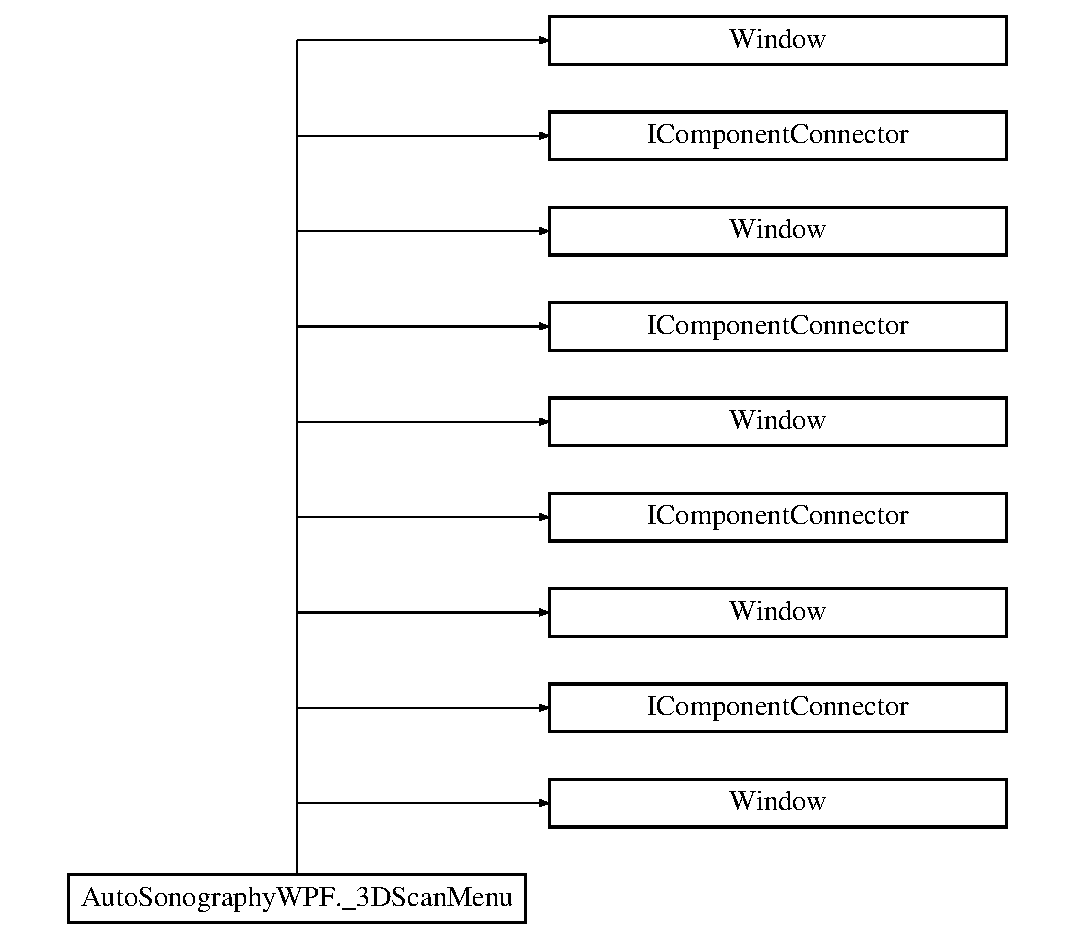
\includegraphics[height=10.000000cm]{class_auto_sonography_w_p_f_1_1__3_d_scan_menu}
\end{center}
\end{figure}
\subsection*{Public Member Functions}
\begin{DoxyCompactItemize}
\item 
void \hyperlink{class_auto_sonography_w_p_f_1_1__3_d_scan_menu_a5e15f9a4094b27b93e34a8c3760db6a5}{Initialize\+Component} ()
\begin{DoxyCompactList}\small\item\em Initialize\+Component \end{DoxyCompactList}\item 
void \hyperlink{class_auto_sonography_w_p_f_1_1__3_d_scan_menu_a5e15f9a4094b27b93e34a8c3760db6a5}{Initialize\+Component} ()
\begin{DoxyCompactList}\small\item\em Initialize\+Component \end{DoxyCompactList}\item 
void \hyperlink{class_auto_sonography_w_p_f_1_1__3_d_scan_menu_a5e15f9a4094b27b93e34a8c3760db6a5}{Initialize\+Component} ()
\begin{DoxyCompactList}\small\item\em Initialize\+Component \end{DoxyCompactList}\item 
void \hyperlink{class_auto_sonography_w_p_f_1_1__3_d_scan_menu_a5e15f9a4094b27b93e34a8c3760db6a5}{Initialize\+Component} ()
\begin{DoxyCompactList}\small\item\em Initialize\+Component \end{DoxyCompactList}\end{DoxyCompactItemize}


\subsection{Detailed Description}
Interaction logic for \+\_\+3\+D\+Scan\+Menu.\+xaml 

\hyperlink{class_auto_sonography_w_p_f_1_1__3_d_scan_menu}{\+\_\+3\+D\+Scan\+Menu} 

\subsection{Member Function Documentation}
\hypertarget{class_auto_sonography_w_p_f_1_1__3_d_scan_menu_a5e15f9a4094b27b93e34a8c3760db6a5}{}\label{class_auto_sonography_w_p_f_1_1__3_d_scan_menu_a5e15f9a4094b27b93e34a8c3760db6a5} 
\index{Auto\+Sonography\+W\+P\+F\+::\+\_\+3\+D\+Scan\+Menu@{Auto\+Sonography\+W\+P\+F\+::\+\_\+3\+D\+Scan\+Menu}!Initialize\+Component@{Initialize\+Component}}
\index{Initialize\+Component@{Initialize\+Component}!Auto\+Sonography\+W\+P\+F\+::\+\_\+3\+D\+Scan\+Menu@{Auto\+Sonography\+W\+P\+F\+::\+\_\+3\+D\+Scan\+Menu}}
\subsubsection{\texorpdfstring{Initialize\+Component()}{InitializeComponent()}\hspace{0.1cm}{\footnotesize\ttfamily [1/4]}}
{\footnotesize\ttfamily void Auto\+Sonography\+W\+P\+F.\+\_\+3\+D\+Scan\+Menu.\+Initialize\+Component (\begin{DoxyParamCaption}{ }\end{DoxyParamCaption})}



Initialize\+Component 

\hypertarget{class_auto_sonography_w_p_f_1_1__3_d_scan_menu_a5e15f9a4094b27b93e34a8c3760db6a5}{}\label{class_auto_sonography_w_p_f_1_1__3_d_scan_menu_a5e15f9a4094b27b93e34a8c3760db6a5} 
\index{Auto\+Sonography\+W\+P\+F\+::\+\_\+3\+D\+Scan\+Menu@{Auto\+Sonography\+W\+P\+F\+::\+\_\+3\+D\+Scan\+Menu}!Initialize\+Component@{Initialize\+Component}}
\index{Initialize\+Component@{Initialize\+Component}!Auto\+Sonography\+W\+P\+F\+::\+\_\+3\+D\+Scan\+Menu@{Auto\+Sonography\+W\+P\+F\+::\+\_\+3\+D\+Scan\+Menu}}
\subsubsection{\texorpdfstring{Initialize\+Component()}{InitializeComponent()}\hspace{0.1cm}{\footnotesize\ttfamily [2/4]}}
{\footnotesize\ttfamily void Auto\+Sonography\+W\+P\+F.\+\_\+3\+D\+Scan\+Menu.\+Initialize\+Component (\begin{DoxyParamCaption}{ }\end{DoxyParamCaption})}



Initialize\+Component 

\hypertarget{class_auto_sonography_w_p_f_1_1__3_d_scan_menu_a5e15f9a4094b27b93e34a8c3760db6a5}{}\label{class_auto_sonography_w_p_f_1_1__3_d_scan_menu_a5e15f9a4094b27b93e34a8c3760db6a5} 
\index{Auto\+Sonography\+W\+P\+F\+::\+\_\+3\+D\+Scan\+Menu@{Auto\+Sonography\+W\+P\+F\+::\+\_\+3\+D\+Scan\+Menu}!Initialize\+Component@{Initialize\+Component}}
\index{Initialize\+Component@{Initialize\+Component}!Auto\+Sonography\+W\+P\+F\+::\+\_\+3\+D\+Scan\+Menu@{Auto\+Sonography\+W\+P\+F\+::\+\_\+3\+D\+Scan\+Menu}}
\subsubsection{\texorpdfstring{Initialize\+Component()}{InitializeComponent()}\hspace{0.1cm}{\footnotesize\ttfamily [3/4]}}
{\footnotesize\ttfamily void Auto\+Sonography\+W\+P\+F.\+\_\+3\+D\+Scan\+Menu.\+Initialize\+Component (\begin{DoxyParamCaption}{ }\end{DoxyParamCaption})}



Initialize\+Component 

\hypertarget{class_auto_sonography_w_p_f_1_1__3_d_scan_menu_a5e15f9a4094b27b93e34a8c3760db6a5}{}\label{class_auto_sonography_w_p_f_1_1__3_d_scan_menu_a5e15f9a4094b27b93e34a8c3760db6a5} 
\index{Auto\+Sonography\+W\+P\+F\+::\+\_\+3\+D\+Scan\+Menu@{Auto\+Sonography\+W\+P\+F\+::\+\_\+3\+D\+Scan\+Menu}!Initialize\+Component@{Initialize\+Component}}
\index{Initialize\+Component@{Initialize\+Component}!Auto\+Sonography\+W\+P\+F\+::\+\_\+3\+D\+Scan\+Menu@{Auto\+Sonography\+W\+P\+F\+::\+\_\+3\+D\+Scan\+Menu}}
\subsubsection{\texorpdfstring{Initialize\+Component()}{InitializeComponent()}\hspace{0.1cm}{\footnotesize\ttfamily [4/4]}}
{\footnotesize\ttfamily void Auto\+Sonography\+W\+P\+F.\+\_\+3\+D\+Scan\+Menu.\+Initialize\+Component (\begin{DoxyParamCaption}{ }\end{DoxyParamCaption})}



Initialize\+Component 



The documentation for this class was generated from the following files\+:\begin{DoxyCompactItemize}
\item 
Auto\+Sonography\+W\+P\+F/3\+D\+Scan\+Menu.\+xaml.\+cs\item 
Auto\+Sonography\+W\+P\+F/obj/\+Debug/3\+D\+Scan\+Menu.\+g.\+cs\item 
Auto\+Sonography\+W\+P\+F/obj/\+Debug/3\+D\+Scan\+Menu.\+g.\+i.\+cs\end{DoxyCompactItemize}

\hypertarget{class_robo_library_1_1_analyzer}{}\section{Robo\+Library.\+Analyzer Class Reference}
\label{class_robo_library_1_1_analyzer}\index{Robo\+Library.\+Analyzer@{Robo\+Library.\+Analyzer}}
Inheritance diagram for Robo\+Library.\+Analyzer\+:\begin{figure}[H]
\begin{center}
\leavevmode
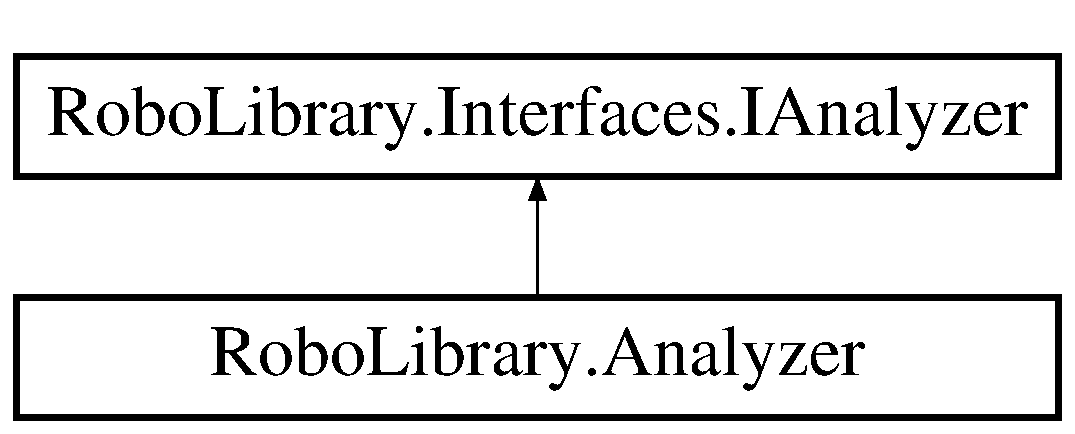
\includegraphics[height=2.000000cm]{class_robo_library_1_1_analyzer}
\end{center}
\end{figure}
\subsection*{Public Member Functions}
\begin{DoxyCompactItemize}
\item 
delegate void \hyperlink{class_robo_library_1_1_analyzer_a232f56c61a30de1de9e27021bf5dc77b}{Actual\+U\+R\+Pose\+Event\+Handler} (\hyperlink{class_robo_library_1_1_u_r_pose}{U\+R\+Pose} a\+Pose)
\begin{DoxyCompactList}\small\item\em Actual UR pose event. This event is called when a new pose is received from the socket stream.\end{DoxyCompactList}\item 
delegate void \hyperlink{class_robo_library_1_1_analyzer_a985396dd045b907a73d7b627b9bd07dc}{Robot\+Message\+Event\+Handler} (Robot\+Message rob\+Msg)
\begin{DoxyCompactList}\small\item\em Robot Message event. This event is called when a new robot message is received from the UR socket stream.\end{DoxyCompactList}\item 
delegate void \hyperlink{class_robo_library_1_1_analyzer_aa1d0cf635115d275b8488aab662610fa}{Robot\+Mode\+Event\+Handler} (string robot\+Mode, string control\+Mode)
\begin{DoxyCompactList}\small\item\em Robot mode event. This event is called when a new robot mode is received from the socket stream.\end{DoxyCompactList}\item 
delegate void \hyperlink{class_robo_library_1_1_analyzer_a6d2960ef27111be171f8c9d6a7d2a058}{Tool\+Mode\+Event\+Handler} (string tool\+Mode)
\begin{DoxyCompactList}\small\item\em Tool mode event. This event is called when a new tool mode is received from the socket stream.\end{DoxyCompactList}\item 
delegate void \hyperlink{class_robo_library_1_1_analyzer_ae03a29ceaec0141398e05cba9cbfba4d}{Safety\+Mode\+Event\+Handler} (string safety\+Mode)
\begin{DoxyCompactList}\small\item\em Safety mode event. This event is called when a new safety mode is received from the socket stream.\end{DoxyCompactList}\item 
\hyperlink{class_robo_library_1_1_analyzer_a2a0c69716b9a8467c56dc8fafcb2fa16}{Analyzer} ()
\begin{DoxyCompactList}\small\item\em Constructor to create instance of Analyse\+U\+R\+Data and instantiate the different modes.\end{DoxyCompactList}\item 
void \hyperlink{class_robo_library_1_1_analyzer_a61fcaef4370cb9a47b12d7cdaf926768}{Read\+U\+R\+Data} (byte\mbox{[}$\,$\mbox{]} data)
\begin{DoxyCompactList}\small\item\em Analyses the data received from the UR socket stream on port 30002.\end{DoxyCompactList}\end{DoxyCompactItemize}
\subsection*{Events}
\begin{DoxyCompactItemize}
\item 
static \hyperlink{class_robo_library_1_1_analyzer_a232f56c61a30de1de9e27021bf5dc77b}{Actual\+U\+R\+Pose\+Event\+Handler} \hyperlink{class_robo_library_1_1_analyzer_a5295d61bea6f0f95d4d7cf6a121efaec}{On\+Actual\+U\+R\+Pose}
\begin{DoxyCompactList}\small\item\em Actual UR pose event. This event is called when a new pose is received from the socket stream.\end{DoxyCompactList}\item 
static \hyperlink{class_robo_library_1_1_analyzer_a985396dd045b907a73d7b627b9bd07dc}{Robot\+Message\+Event\+Handler} \hyperlink{class_robo_library_1_1_analyzer_ad2f4496aa598c9e9a8380c484aacdb5d}{On\+Robot\+Message}
\begin{DoxyCompactList}\small\item\em Robot Message event. This event is called when a new robot message is received from the UR socket stream.\end{DoxyCompactList}\item 
static \hyperlink{class_robo_library_1_1_analyzer_aa1d0cf635115d275b8488aab662610fa}{Robot\+Mode\+Event\+Handler} \hyperlink{class_robo_library_1_1_analyzer_a18356690d4cc11656007057cca93f278}{On\+Robot\+Mode}
\begin{DoxyCompactList}\small\item\em Robot mode event. This event is called when a new robot mode is received from the socket stream.\end{DoxyCompactList}\item 
static \hyperlink{class_robo_library_1_1_analyzer_a6d2960ef27111be171f8c9d6a7d2a058}{Tool\+Mode\+Event\+Handler} \hyperlink{class_robo_library_1_1_analyzer_aed192ad0336a1115cf10504bcf5abfc5}{On\+Tool\+Mode}
\begin{DoxyCompactList}\small\item\em Tool mode event. This event is called when a new tool mode is received from the socket stream.\end{DoxyCompactList}\item 
static \hyperlink{class_robo_library_1_1_analyzer_ae03a29ceaec0141398e05cba9cbfba4d}{Safety\+Mode\+Event\+Handler} \hyperlink{class_robo_library_1_1_analyzer_a77e89608a449d5ae30eadf9b2d1ed8e3}{On\+Safety\+Mode}
\begin{DoxyCompactList}\small\item\em Safety mode event. This event is called when a new safety mode is received from the socket stream.\end{DoxyCompactList}\end{DoxyCompactItemize}


\subsection{Constructor \& Destructor Documentation}
\hypertarget{class_robo_library_1_1_analyzer_a2a0c69716b9a8467c56dc8fafcb2fa16}{}\label{class_robo_library_1_1_analyzer_a2a0c69716b9a8467c56dc8fafcb2fa16} 
\index{Robo\+Library\+::\+Analyzer@{Robo\+Library\+::\+Analyzer}!Analyzer@{Analyzer}}
\index{Analyzer@{Analyzer}!Robo\+Library\+::\+Analyzer@{Robo\+Library\+::\+Analyzer}}
\subsubsection{\texorpdfstring{Analyzer()}{Analyzer()}}
{\footnotesize\ttfamily Robo\+Library.\+Analyzer.\+Analyzer (\begin{DoxyParamCaption}{ }\end{DoxyParamCaption})}



Constructor to create instance of Analyse\+U\+R\+Data and instantiate the different modes.



\subsection{Member Function Documentation}
\hypertarget{class_robo_library_1_1_analyzer_a232f56c61a30de1de9e27021bf5dc77b}{}\label{class_robo_library_1_1_analyzer_a232f56c61a30de1de9e27021bf5dc77b} 
\index{Robo\+Library\+::\+Analyzer@{Robo\+Library\+::\+Analyzer}!Actual\+U\+R\+Pose\+Event\+Handler@{Actual\+U\+R\+Pose\+Event\+Handler}}
\index{Actual\+U\+R\+Pose\+Event\+Handler@{Actual\+U\+R\+Pose\+Event\+Handler}!Robo\+Library\+::\+Analyzer@{Robo\+Library\+::\+Analyzer}}
\subsubsection{\texorpdfstring{Actual\+U\+R\+Pose\+Event\+Handler()}{ActualURPoseEventHandler()}}
{\footnotesize\ttfamily delegate void Robo\+Library.\+Analyzer.\+Actual\+U\+R\+Pose\+Event\+Handler (\begin{DoxyParamCaption}\item[{\hyperlink{class_robo_library_1_1_u_r_pose}{U\+R\+Pose}}]{a\+Pose }\end{DoxyParamCaption})}



Actual UR pose event. This event is called when a new pose is received from the socket stream.

\hypertarget{class_robo_library_1_1_analyzer_a61fcaef4370cb9a47b12d7cdaf926768}{}\label{class_robo_library_1_1_analyzer_a61fcaef4370cb9a47b12d7cdaf926768} 
\index{Robo\+Library\+::\+Analyzer@{Robo\+Library\+::\+Analyzer}!Read\+U\+R\+Data@{Read\+U\+R\+Data}}
\index{Read\+U\+R\+Data@{Read\+U\+R\+Data}!Robo\+Library\+::\+Analyzer@{Robo\+Library\+::\+Analyzer}}
\subsubsection{\texorpdfstring{Read\+U\+R\+Data()}{ReadURData()}}
{\footnotesize\ttfamily void Robo\+Library.\+Analyzer.\+Read\+U\+R\+Data (\begin{DoxyParamCaption}\item[{byte \mbox{[}$\,$\mbox{]}}]{data }\end{DoxyParamCaption})}



Analyses the data received from the UR socket stream on port 30002.


\begin{DoxyParams}{Parameters}
{\em data} & Byte array received on the socket stream.\\
\hline
\end{DoxyParams}


Implements \hyperlink{interface_robo_library_1_1_interfaces_1_1_i_analyzer}{Robo\+Library.\+Interfaces.\+I\+Analyzer}.

\hypertarget{class_robo_library_1_1_analyzer_a985396dd045b907a73d7b627b9bd07dc}{}\label{class_robo_library_1_1_analyzer_a985396dd045b907a73d7b627b9bd07dc} 
\index{Robo\+Library\+::\+Analyzer@{Robo\+Library\+::\+Analyzer}!Robot\+Message\+Event\+Handler@{Robot\+Message\+Event\+Handler}}
\index{Robot\+Message\+Event\+Handler@{Robot\+Message\+Event\+Handler}!Robo\+Library\+::\+Analyzer@{Robo\+Library\+::\+Analyzer}}
\subsubsection{\texorpdfstring{Robot\+Message\+Event\+Handler()}{RobotMessageEventHandler()}}
{\footnotesize\ttfamily delegate void Robo\+Library.\+Analyzer.\+Robot\+Message\+Event\+Handler (\begin{DoxyParamCaption}\item[{Robot\+Message}]{rob\+Msg }\end{DoxyParamCaption})}



Robot Message event. This event is called when a new robot message is received from the UR socket stream.

\hypertarget{class_robo_library_1_1_analyzer_aa1d0cf635115d275b8488aab662610fa}{}\label{class_robo_library_1_1_analyzer_aa1d0cf635115d275b8488aab662610fa} 
\index{Robo\+Library\+::\+Analyzer@{Robo\+Library\+::\+Analyzer}!Robot\+Mode\+Event\+Handler@{Robot\+Mode\+Event\+Handler}}
\index{Robot\+Mode\+Event\+Handler@{Robot\+Mode\+Event\+Handler}!Robo\+Library\+::\+Analyzer@{Robo\+Library\+::\+Analyzer}}
\subsubsection{\texorpdfstring{Robot\+Mode\+Event\+Handler()}{RobotModeEventHandler()}}
{\footnotesize\ttfamily delegate void Robo\+Library.\+Analyzer.\+Robot\+Mode\+Event\+Handler (\begin{DoxyParamCaption}\item[{string}]{robot\+Mode,  }\item[{string}]{control\+Mode }\end{DoxyParamCaption})}



Robot mode event. This event is called when a new robot mode is received from the socket stream.

\hypertarget{class_robo_library_1_1_analyzer_ae03a29ceaec0141398e05cba9cbfba4d}{}\label{class_robo_library_1_1_analyzer_ae03a29ceaec0141398e05cba9cbfba4d} 
\index{Robo\+Library\+::\+Analyzer@{Robo\+Library\+::\+Analyzer}!Safety\+Mode\+Event\+Handler@{Safety\+Mode\+Event\+Handler}}
\index{Safety\+Mode\+Event\+Handler@{Safety\+Mode\+Event\+Handler}!Robo\+Library\+::\+Analyzer@{Robo\+Library\+::\+Analyzer}}
\subsubsection{\texorpdfstring{Safety\+Mode\+Event\+Handler()}{SafetyModeEventHandler()}}
{\footnotesize\ttfamily delegate void Robo\+Library.\+Analyzer.\+Safety\+Mode\+Event\+Handler (\begin{DoxyParamCaption}\item[{string}]{safety\+Mode }\end{DoxyParamCaption})}



Safety mode event. This event is called when a new safety mode is received from the socket stream.

\hypertarget{class_robo_library_1_1_analyzer_a6d2960ef27111be171f8c9d6a7d2a058}{}\label{class_robo_library_1_1_analyzer_a6d2960ef27111be171f8c9d6a7d2a058} 
\index{Robo\+Library\+::\+Analyzer@{Robo\+Library\+::\+Analyzer}!Tool\+Mode\+Event\+Handler@{Tool\+Mode\+Event\+Handler}}
\index{Tool\+Mode\+Event\+Handler@{Tool\+Mode\+Event\+Handler}!Robo\+Library\+::\+Analyzer@{Robo\+Library\+::\+Analyzer}}
\subsubsection{\texorpdfstring{Tool\+Mode\+Event\+Handler()}{ToolModeEventHandler()}}
{\footnotesize\ttfamily delegate void Robo\+Library.\+Analyzer.\+Tool\+Mode\+Event\+Handler (\begin{DoxyParamCaption}\item[{string}]{tool\+Mode }\end{DoxyParamCaption})}



Tool mode event. This event is called when a new tool mode is received from the socket stream.



\subsection{Event Documentation}
\hypertarget{class_robo_library_1_1_analyzer_a5295d61bea6f0f95d4d7cf6a121efaec}{}\label{class_robo_library_1_1_analyzer_a5295d61bea6f0f95d4d7cf6a121efaec} 
\index{Robo\+Library\+::\+Analyzer@{Robo\+Library\+::\+Analyzer}!On\+Actual\+U\+R\+Pose@{On\+Actual\+U\+R\+Pose}}
\index{On\+Actual\+U\+R\+Pose@{On\+Actual\+U\+R\+Pose}!Robo\+Library\+::\+Analyzer@{Robo\+Library\+::\+Analyzer}}
\subsubsection{\texorpdfstring{On\+Actual\+U\+R\+Pose}{OnActualURPose}}
{\footnotesize\ttfamily \hyperlink{class_robo_library_1_1_analyzer_a232f56c61a30de1de9e27021bf5dc77b}{Actual\+U\+R\+Pose\+Event\+Handler} Robo\+Library.\+Analyzer.\+On\+Actual\+U\+R\+Pose\hspace{0.3cm}{\ttfamily [static]}}



Actual UR pose event. This event is called when a new pose is received from the socket stream.

\hypertarget{class_robo_library_1_1_analyzer_ad2f4496aa598c9e9a8380c484aacdb5d}{}\label{class_robo_library_1_1_analyzer_ad2f4496aa598c9e9a8380c484aacdb5d} 
\index{Robo\+Library\+::\+Analyzer@{Robo\+Library\+::\+Analyzer}!On\+Robot\+Message@{On\+Robot\+Message}}
\index{On\+Robot\+Message@{On\+Robot\+Message}!Robo\+Library\+::\+Analyzer@{Robo\+Library\+::\+Analyzer}}
\subsubsection{\texorpdfstring{On\+Robot\+Message}{OnRobotMessage}}
{\footnotesize\ttfamily \hyperlink{class_robo_library_1_1_analyzer_a985396dd045b907a73d7b627b9bd07dc}{Robot\+Message\+Event\+Handler} Robo\+Library.\+Analyzer.\+On\+Robot\+Message\hspace{0.3cm}{\ttfamily [static]}}



Robot Message event. This event is called when a new robot message is received from the UR socket stream.

\hypertarget{class_robo_library_1_1_analyzer_a18356690d4cc11656007057cca93f278}{}\label{class_robo_library_1_1_analyzer_a18356690d4cc11656007057cca93f278} 
\index{Robo\+Library\+::\+Analyzer@{Robo\+Library\+::\+Analyzer}!On\+Robot\+Mode@{On\+Robot\+Mode}}
\index{On\+Robot\+Mode@{On\+Robot\+Mode}!Robo\+Library\+::\+Analyzer@{Robo\+Library\+::\+Analyzer}}
\subsubsection{\texorpdfstring{On\+Robot\+Mode}{OnRobotMode}}
{\footnotesize\ttfamily \hyperlink{class_robo_library_1_1_analyzer_aa1d0cf635115d275b8488aab662610fa}{Robot\+Mode\+Event\+Handler} Robo\+Library.\+Analyzer.\+On\+Robot\+Mode\hspace{0.3cm}{\ttfamily [static]}}



Robot mode event. This event is called when a new robot mode is received from the socket stream.

\hypertarget{class_robo_library_1_1_analyzer_a77e89608a449d5ae30eadf9b2d1ed8e3}{}\label{class_robo_library_1_1_analyzer_a77e89608a449d5ae30eadf9b2d1ed8e3} 
\index{Robo\+Library\+::\+Analyzer@{Robo\+Library\+::\+Analyzer}!On\+Safety\+Mode@{On\+Safety\+Mode}}
\index{On\+Safety\+Mode@{On\+Safety\+Mode}!Robo\+Library\+::\+Analyzer@{Robo\+Library\+::\+Analyzer}}
\subsubsection{\texorpdfstring{On\+Safety\+Mode}{OnSafetyMode}}
{\footnotesize\ttfamily \hyperlink{class_robo_library_1_1_analyzer_ae03a29ceaec0141398e05cba9cbfba4d}{Safety\+Mode\+Event\+Handler} Robo\+Library.\+Analyzer.\+On\+Safety\+Mode\hspace{0.3cm}{\ttfamily [static]}}



Safety mode event. This event is called when a new safety mode is received from the socket stream.

\hypertarget{class_robo_library_1_1_analyzer_aed192ad0336a1115cf10504bcf5abfc5}{}\label{class_robo_library_1_1_analyzer_aed192ad0336a1115cf10504bcf5abfc5} 
\index{Robo\+Library\+::\+Analyzer@{Robo\+Library\+::\+Analyzer}!On\+Tool\+Mode@{On\+Tool\+Mode}}
\index{On\+Tool\+Mode@{On\+Tool\+Mode}!Robo\+Library\+::\+Analyzer@{Robo\+Library\+::\+Analyzer}}
\subsubsection{\texorpdfstring{On\+Tool\+Mode}{OnToolMode}}
{\footnotesize\ttfamily \hyperlink{class_robo_library_1_1_analyzer_a6d2960ef27111be171f8c9d6a7d2a058}{Tool\+Mode\+Event\+Handler} Robo\+Library.\+Analyzer.\+On\+Tool\+Mode\hspace{0.3cm}{\ttfamily [static]}}



Tool mode event. This event is called when a new tool mode is received from the socket stream.



The documentation for this class was generated from the following file\+:\begin{DoxyCompactItemize}
\item 
Robo\+Library/Analyzer.\+cs\end{DoxyCompactItemize}

\hypertarget{class_auto_sonography_w_p_f_1_1_app}{}\section{Auto\+Sonography\+W\+P\+F.\+App Class Reference}
\label{class_auto_sonography_w_p_f_1_1_app}\index{Auto\+Sonography\+W\+P\+F.\+App@{Auto\+Sonography\+W\+P\+F.\+App}}


Interaction logic for App.\+xaml  


Inheritance diagram for Auto\+Sonography\+W\+P\+F.\+App\+:\begin{figure}[H]
\begin{center}
\leavevmode
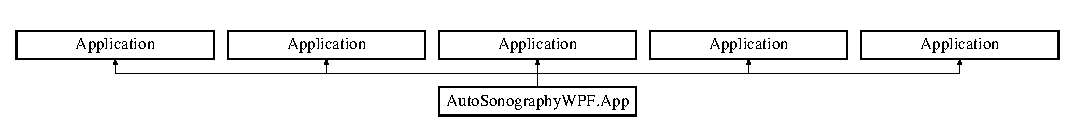
\includegraphics[height=1.325444cm]{class_auto_sonography_w_p_f_1_1_app}
\end{center}
\end{figure}
\subsection*{Public Member Functions}
\begin{DoxyCompactItemize}
\item 
void \hyperlink{class_auto_sonography_w_p_f_1_1_app_a5878d4ccc5b6d4f1343b839cfa9babbb}{Initialize\+Component} ()
\begin{DoxyCompactList}\small\item\em Initialize\+Component \end{DoxyCompactList}\item 
void \hyperlink{class_auto_sonography_w_p_f_1_1_app_a5878d4ccc5b6d4f1343b839cfa9babbb}{Initialize\+Component} ()
\begin{DoxyCompactList}\small\item\em Initialize\+Component \end{DoxyCompactList}\item 
void \hyperlink{class_auto_sonography_w_p_f_1_1_app_a5878d4ccc5b6d4f1343b839cfa9babbb}{Initialize\+Component} ()
\begin{DoxyCompactList}\small\item\em Initialize\+Component \end{DoxyCompactList}\item 
void \hyperlink{class_auto_sonography_w_p_f_1_1_app_a5878d4ccc5b6d4f1343b839cfa9babbb}{Initialize\+Component} ()
\begin{DoxyCompactList}\small\item\em Initialize\+Component \end{DoxyCompactList}\end{DoxyCompactItemize}
\subsection*{Static Public Member Functions}
\begin{DoxyCompactItemize}
\item 
static void \hyperlink{class_auto_sonography_w_p_f_1_1_app_a78f9df146a506989aad70cdf7863bd1e}{Main} ()
\begin{DoxyCompactList}\small\item\em Application Entry Point. \end{DoxyCompactList}\item 
static void \hyperlink{class_auto_sonography_w_p_f_1_1_app_a78f9df146a506989aad70cdf7863bd1e}{Main} ()
\begin{DoxyCompactList}\small\item\em Application Entry Point. \end{DoxyCompactList}\item 
static void \hyperlink{class_auto_sonography_w_p_f_1_1_app_a78f9df146a506989aad70cdf7863bd1e}{Main} ()
\begin{DoxyCompactList}\small\item\em Application Entry Point. \end{DoxyCompactList}\item 
static void \hyperlink{class_auto_sonography_w_p_f_1_1_app_a78f9df146a506989aad70cdf7863bd1e}{Main} ()
\begin{DoxyCompactList}\small\item\em Application Entry Point. \end{DoxyCompactList}\end{DoxyCompactItemize}


\subsection{Detailed Description}
Interaction logic for App.\+xaml 

\hyperlink{class_auto_sonography_w_p_f_1_1_app}{App} 

\subsection{Member Function Documentation}
\hypertarget{class_auto_sonography_w_p_f_1_1_app_a5878d4ccc5b6d4f1343b839cfa9babbb}{}\label{class_auto_sonography_w_p_f_1_1_app_a5878d4ccc5b6d4f1343b839cfa9babbb} 
\index{Auto\+Sonography\+W\+P\+F\+::\+App@{Auto\+Sonography\+W\+P\+F\+::\+App}!Initialize\+Component@{Initialize\+Component}}
\index{Initialize\+Component@{Initialize\+Component}!Auto\+Sonography\+W\+P\+F\+::\+App@{Auto\+Sonography\+W\+P\+F\+::\+App}}
\subsubsection{\texorpdfstring{Initialize\+Component()}{InitializeComponent()}\hspace{0.1cm}{\footnotesize\ttfamily [1/4]}}
{\footnotesize\ttfamily void Auto\+Sonography\+W\+P\+F.\+App.\+Initialize\+Component (\begin{DoxyParamCaption}{ }\end{DoxyParamCaption})}



Initialize\+Component 

\hypertarget{class_auto_sonography_w_p_f_1_1_app_a5878d4ccc5b6d4f1343b839cfa9babbb}{}\label{class_auto_sonography_w_p_f_1_1_app_a5878d4ccc5b6d4f1343b839cfa9babbb} 
\index{Auto\+Sonography\+W\+P\+F\+::\+App@{Auto\+Sonography\+W\+P\+F\+::\+App}!Initialize\+Component@{Initialize\+Component}}
\index{Initialize\+Component@{Initialize\+Component}!Auto\+Sonography\+W\+P\+F\+::\+App@{Auto\+Sonography\+W\+P\+F\+::\+App}}
\subsubsection{\texorpdfstring{Initialize\+Component()}{InitializeComponent()}\hspace{0.1cm}{\footnotesize\ttfamily [2/4]}}
{\footnotesize\ttfamily void Auto\+Sonography\+W\+P\+F.\+App.\+Initialize\+Component (\begin{DoxyParamCaption}{ }\end{DoxyParamCaption})}



Initialize\+Component 

\hypertarget{class_auto_sonography_w_p_f_1_1_app_a5878d4ccc5b6d4f1343b839cfa9babbb}{}\label{class_auto_sonography_w_p_f_1_1_app_a5878d4ccc5b6d4f1343b839cfa9babbb} 
\index{Auto\+Sonography\+W\+P\+F\+::\+App@{Auto\+Sonography\+W\+P\+F\+::\+App}!Initialize\+Component@{Initialize\+Component}}
\index{Initialize\+Component@{Initialize\+Component}!Auto\+Sonography\+W\+P\+F\+::\+App@{Auto\+Sonography\+W\+P\+F\+::\+App}}
\subsubsection{\texorpdfstring{Initialize\+Component()}{InitializeComponent()}\hspace{0.1cm}{\footnotesize\ttfamily [3/4]}}
{\footnotesize\ttfamily void Auto\+Sonography\+W\+P\+F.\+App.\+Initialize\+Component (\begin{DoxyParamCaption}{ }\end{DoxyParamCaption})}



Initialize\+Component 

\hypertarget{class_auto_sonography_w_p_f_1_1_app_a5878d4ccc5b6d4f1343b839cfa9babbb}{}\label{class_auto_sonography_w_p_f_1_1_app_a5878d4ccc5b6d4f1343b839cfa9babbb} 
\index{Auto\+Sonography\+W\+P\+F\+::\+App@{Auto\+Sonography\+W\+P\+F\+::\+App}!Initialize\+Component@{Initialize\+Component}}
\index{Initialize\+Component@{Initialize\+Component}!Auto\+Sonography\+W\+P\+F\+::\+App@{Auto\+Sonography\+W\+P\+F\+::\+App}}
\subsubsection{\texorpdfstring{Initialize\+Component()}{InitializeComponent()}\hspace{0.1cm}{\footnotesize\ttfamily [4/4]}}
{\footnotesize\ttfamily void Auto\+Sonography\+W\+P\+F.\+App.\+Initialize\+Component (\begin{DoxyParamCaption}{ }\end{DoxyParamCaption})}



Initialize\+Component 

\hypertarget{class_auto_sonography_w_p_f_1_1_app_a78f9df146a506989aad70cdf7863bd1e}{}\label{class_auto_sonography_w_p_f_1_1_app_a78f9df146a506989aad70cdf7863bd1e} 
\index{Auto\+Sonography\+W\+P\+F\+::\+App@{Auto\+Sonography\+W\+P\+F\+::\+App}!Main@{Main}}
\index{Main@{Main}!Auto\+Sonography\+W\+P\+F\+::\+App@{Auto\+Sonography\+W\+P\+F\+::\+App}}
\subsubsection{\texorpdfstring{Main()}{Main()}\hspace{0.1cm}{\footnotesize\ttfamily [1/4]}}
{\footnotesize\ttfamily static void Auto\+Sonography\+W\+P\+F.\+App.\+Main (\begin{DoxyParamCaption}{ }\end{DoxyParamCaption})\hspace{0.3cm}{\ttfamily [static]}}



Application Entry Point. 

\hypertarget{class_auto_sonography_w_p_f_1_1_app_a78f9df146a506989aad70cdf7863bd1e}{}\label{class_auto_sonography_w_p_f_1_1_app_a78f9df146a506989aad70cdf7863bd1e} 
\index{Auto\+Sonography\+W\+P\+F\+::\+App@{Auto\+Sonography\+W\+P\+F\+::\+App}!Main@{Main}}
\index{Main@{Main}!Auto\+Sonography\+W\+P\+F\+::\+App@{Auto\+Sonography\+W\+P\+F\+::\+App}}
\subsubsection{\texorpdfstring{Main()}{Main()}\hspace{0.1cm}{\footnotesize\ttfamily [2/4]}}
{\footnotesize\ttfamily static void Auto\+Sonography\+W\+P\+F.\+App.\+Main (\begin{DoxyParamCaption}{ }\end{DoxyParamCaption})\hspace{0.3cm}{\ttfamily [static]}}



Application Entry Point. 

\hypertarget{class_auto_sonography_w_p_f_1_1_app_a78f9df146a506989aad70cdf7863bd1e}{}\label{class_auto_sonography_w_p_f_1_1_app_a78f9df146a506989aad70cdf7863bd1e} 
\index{Auto\+Sonography\+W\+P\+F\+::\+App@{Auto\+Sonography\+W\+P\+F\+::\+App}!Main@{Main}}
\index{Main@{Main}!Auto\+Sonography\+W\+P\+F\+::\+App@{Auto\+Sonography\+W\+P\+F\+::\+App}}
\subsubsection{\texorpdfstring{Main()}{Main()}\hspace{0.1cm}{\footnotesize\ttfamily [3/4]}}
{\footnotesize\ttfamily static void Auto\+Sonography\+W\+P\+F.\+App.\+Main (\begin{DoxyParamCaption}{ }\end{DoxyParamCaption})\hspace{0.3cm}{\ttfamily [static]}}



Application Entry Point. 

\hypertarget{class_auto_sonography_w_p_f_1_1_app_a78f9df146a506989aad70cdf7863bd1e}{}\label{class_auto_sonography_w_p_f_1_1_app_a78f9df146a506989aad70cdf7863bd1e} 
\index{Auto\+Sonography\+W\+P\+F\+::\+App@{Auto\+Sonography\+W\+P\+F\+::\+App}!Main@{Main}}
\index{Main@{Main}!Auto\+Sonography\+W\+P\+F\+::\+App@{Auto\+Sonography\+W\+P\+F\+::\+App}}
\subsubsection{\texorpdfstring{Main()}{Main()}\hspace{0.1cm}{\footnotesize\ttfamily [4/4]}}
{\footnotesize\ttfamily static void Auto\+Sonography\+W\+P\+F.\+App.\+Main (\begin{DoxyParamCaption}{ }\end{DoxyParamCaption})\hspace{0.3cm}{\ttfamily [static]}}



Application Entry Point. 



The documentation for this class was generated from the following files\+:\begin{DoxyCompactItemize}
\item 
Auto\+Sonography\+W\+P\+F/App.\+xaml.\+cs\item 
Auto\+Sonography\+W\+P\+F/obj/\+Debug/App.\+g.\+cs\item 
Auto\+Sonography\+W\+P\+F/obj/\+Debug/App.\+g.\+i.\+cs\end{DoxyCompactItemize}

\hypertarget{class_robo_library_1_1_camera_to_robot_calibrator}{}\section{Robo\+Library.\+Camera\+To\+Robot\+Calibrator Class Reference}
\label{class_robo_library_1_1_camera_to_robot_calibrator}\index{Robo\+Library.\+Camera\+To\+Robot\+Calibrator@{Robo\+Library.\+Camera\+To\+Robot\+Calibrator}}
\subsection*{Public Member Functions}
\begin{DoxyCompactItemize}
\item 
\hypertarget{class_robo_library_1_1_camera_to_robot_calibrator_a25fdd80bf754a9bb60e710373bb6495d}{}\label{class_robo_library_1_1_camera_to_robot_calibrator_a25fdd80bf754a9bb60e710373bb6495d} 
Color\+Mesh {\bfseries Convert\+To\+Robospace} (Color\+Mesh mesh)
\end{DoxyCompactItemize}
\subsection*{Public Attributes}
\begin{DoxyCompactItemize}
\item 
\hypertarget{class_robo_library_1_1_camera_to_robot_calibrator_a69134a5024ee008aa6999ea2981a8d7c}{}\label{class_robo_library_1_1_camera_to_robot_calibrator_a69134a5024ee008aa6999ea2981a8d7c} 
const float {\bfseries x\+\_\+offset} = 0f
\item 
\hypertarget{class_robo_library_1_1_camera_to_robot_calibrator_a5333e43ca61bba12c4fded9f169b8f05}{}\label{class_robo_library_1_1_camera_to_robot_calibrator_a5333e43ca61bba12c4fded9f169b8f05} 
const float {\bfseries y\+\_\+offset} = 0f
\item 
\hypertarget{class_robo_library_1_1_camera_to_robot_calibrator_ab258ba554892ffda94f04d67483e0213}{}\label{class_robo_library_1_1_camera_to_robot_calibrator_ab258ba554892ffda94f04d67483e0213} 
const float {\bfseries z\+\_\+offset} = 0f
\item 
\hypertarget{class_robo_library_1_1_camera_to_robot_calibrator_a8edffd65a172e18c7bafef8b16cc6444}{}\label{class_robo_library_1_1_camera_to_robot_calibrator_a8edffd65a172e18c7bafef8b16cc6444} 
const float {\bfseries x\+\_\+rotation} = 0f
\item 
\hypertarget{class_robo_library_1_1_camera_to_robot_calibrator_a9ce3105bf68d247fcfad9390da1849f0}{}\label{class_robo_library_1_1_camera_to_robot_calibrator_a9ce3105bf68d247fcfad9390da1849f0} 
const float {\bfseries y\+\_\+rotation} = 0f
\item 
\hypertarget{class_robo_library_1_1_camera_to_robot_calibrator_a023b40704091a0cc34835895299be4b1}{}\label{class_robo_library_1_1_camera_to_robot_calibrator_a023b40704091a0cc34835895299be4b1} 
const float {\bfseries z\+\_\+rotation} = -\/90f
\end{DoxyCompactItemize}


The documentation for this class was generated from the following file\+:\begin{DoxyCompactItemize}
\item 
Robo\+Library/Camera\+To\+Robot\+Calibrator.\+cs\end{DoxyCompactItemize}

\hypertarget{class_computer_vision_library_1_1_color_vertex_slicer}{}\section{Computer\+Vision\+Library.\+Color\+Vertex\+Slicer Class Reference}
\label{class_computer_vision_library_1_1_color_vertex_slicer}\index{Computer\+Vision\+Library.\+Color\+Vertex\+Slicer@{Computer\+Vision\+Library.\+Color\+Vertex\+Slicer}}
\subsection*{Public Member Functions}
\begin{DoxyCompactItemize}
\item 
\hypertarget{class_computer_vision_library_1_1_color_vertex_slicer_a56f877bf8c9dd7e30346b26d96527e65}{}\label{class_computer_vision_library_1_1_color_vertex_slicer_a56f877bf8c9dd7e30346b26d96527e65} 
\hyperlink{class_computer_vision_library_1_1_mesh}{Mesh} {\bfseries Remove\+Undesirables} (\hyperlink{class_computer_vision_library_1_1_mesh}{Mesh} mesh, Color color)
\item 
bool \hyperlink{class_computer_vision_library_1_1_color_vertex_slicer_a0c9a976faaff5db5d7a5aa5c8bc5f1f7}{Is\+Within\+Threshold} (Color check, Color desirable)
\begin{DoxyCompactList}\small\item\em Checks if a color is close to another \end{DoxyCompactList}\end{DoxyCompactItemize}
\subsection*{Public Attributes}
\begin{DoxyCompactItemize}
\item 
readonly byte \hyperlink{class_computer_vision_library_1_1_color_vertex_slicer_a7313d6cee1d46433875b7aa61ec1d36e}{Threshold} = 30
\begin{DoxyCompactList}\small\item\em Inputting R\+GB = 0,0,245 allows the color to be accepted up to 10,10,255 and down to 0,0,235 \end{DoxyCompactList}\end{DoxyCompactItemize}


\subsection{Member Function Documentation}
\hypertarget{class_computer_vision_library_1_1_color_vertex_slicer_a0c9a976faaff5db5d7a5aa5c8bc5f1f7}{}\label{class_computer_vision_library_1_1_color_vertex_slicer_a0c9a976faaff5db5d7a5aa5c8bc5f1f7} 
\index{Computer\+Vision\+Library\+::\+Color\+Vertex\+Slicer@{Computer\+Vision\+Library\+::\+Color\+Vertex\+Slicer}!Is\+Within\+Threshold@{Is\+Within\+Threshold}}
\index{Is\+Within\+Threshold@{Is\+Within\+Threshold}!Computer\+Vision\+Library\+::\+Color\+Vertex\+Slicer@{Computer\+Vision\+Library\+::\+Color\+Vertex\+Slicer}}
\subsubsection{\texorpdfstring{Is\+Within\+Threshold()}{IsWithinThreshold()}}
{\footnotesize\ttfamily bool Computer\+Vision\+Library.\+Color\+Vertex\+Slicer.\+Is\+Within\+Threshold (\begin{DoxyParamCaption}\item[{Color}]{check,  }\item[{Color}]{desirable }\end{DoxyParamCaption})}



Checks if a color is close to another 


\begin{DoxyParams}{Parameters}
{\em check} & The color we\textquotesingle{}re checking\\
\hline
{\em desirable} & The color we\textquotesingle{}re checking up against\\
\hline
\end{DoxyParams}
\begin{DoxyReturn}{Returns}
A boolean describing if it\textquotesingle{}s close or not
\end{DoxyReturn}


\subsection{Member Data Documentation}
\hypertarget{class_computer_vision_library_1_1_color_vertex_slicer_a7313d6cee1d46433875b7aa61ec1d36e}{}\label{class_computer_vision_library_1_1_color_vertex_slicer_a7313d6cee1d46433875b7aa61ec1d36e} 
\index{Computer\+Vision\+Library\+::\+Color\+Vertex\+Slicer@{Computer\+Vision\+Library\+::\+Color\+Vertex\+Slicer}!Threshold@{Threshold}}
\index{Threshold@{Threshold}!Computer\+Vision\+Library\+::\+Color\+Vertex\+Slicer@{Computer\+Vision\+Library\+::\+Color\+Vertex\+Slicer}}
\subsubsection{\texorpdfstring{Threshold}{Threshold}}
{\footnotesize\ttfamily readonly byte Computer\+Vision\+Library.\+Color\+Vertex\+Slicer.\+Threshold = 30}



Inputting R\+GB = 0,0,245 allows the color to be accepted up to 10,10,255 and down to 0,0,235 



The documentation for this class was generated from the following file\+:\begin{DoxyCompactItemize}
\item 
Computer\+Vision\+Library/Color\+Vertex\+Slicer.\+cs\end{DoxyCompactItemize}

\hypertarget{class_computer_vision_library_1_1_computer_vision_master}{}\section{Computer\+Vision\+Library.\+Computer\+Vision\+Master Class Reference}
\label{class_computer_vision_library_1_1_computer_vision_master}\index{Computer\+Vision\+Library.\+Computer\+Vision\+Master@{Computer\+Vision\+Library.\+Computer\+Vision\+Master}}
\subsection*{Public Member Functions}
\begin{DoxyCompactItemize}
\item 
\hypertarget{class_computer_vision_library_1_1_computer_vision_master_ada2dc4f967b6445f15402529fd92f326}{}\label{class_computer_vision_library_1_1_computer_vision_master_ada2dc4f967b6445f15402529fd92f326} 
void {\bfseries Request\+Current\+Image\+As\+Mesh} ()
\item 
\hypertarget{class_computer_vision_library_1_1_computer_vision_master_a68d823632038d891aecda1e59f1435ea}{}\label{class_computer_vision_library_1_1_computer_vision_master_a68d823632038d891aecda1e59f1435ea} 
void {\bfseries Retrieve\+Mesh} (Color\+Mesh mesh)
\end{DoxyCompactItemize}
\subsection*{Public Attributes}
\begin{DoxyCompactItemize}
\item 
\hypertarget{class_computer_vision_library_1_1_computer_vision_master_a458d3174af2f9c2ec669b8cffc1b6ae7}{}\label{class_computer_vision_library_1_1_computer_vision_master_a458d3174af2f9c2ec669b8cffc1b6ae7} 
string {\bfseries Last\+Mesh\+Location}
\end{DoxyCompactItemize}
\subsection*{Properties}
\begin{DoxyCompactItemize}
\item 
\hypertarget{class_computer_vision_library_1_1_computer_vision_master_a474cec41ba592341899c080ba14663eb}{}\label{class_computer_vision_library_1_1_computer_vision_master_a474cec41ba592341899c080ba14663eb} 
static \hyperlink{class_computer_vision_library_1_1_computer_vision_master}{Computer\+Vision\+Master} {\bfseries Instance}\hspace{0.3cm}{\ttfamily  \mbox{[}get\mbox{]}}
\end{DoxyCompactItemize}


The documentation for this class was generated from the following file\+:\begin{DoxyCompactItemize}
\item 
Computer\+Vision\+Library/Computer\+Vision\+Master.\+cs\end{DoxyCompactItemize}

\hypertarget{class_robo_library_1_1_data}{}\section{Robo\+Library.\+Data Class Reference}
\label{class_robo_library_1_1_data}\index{Robo\+Library.\+Data@{Robo\+Library.\+Data}}
\subsection*{Public Member Functions}
\begin{DoxyCompactItemize}
\item 
\hypertarget{class_robo_library_1_1_data_ab82bf5ac661fb88659696f401b1a7037}{}\label{class_robo_library_1_1_data_ab82bf5ac661fb88659696f401b1a7037} 
delegate void {\bfseries Configuration\+Event\+Handler} (bool result)
\item 
\hypertarget{class_robo_library_1_1_data_ab6c5d04b89fa699ceaf7146d536e7c39}{}\label{class_robo_library_1_1_data_ab6c5d04b89fa699ceaf7146d536e7c39} 
delegate void {\bfseries Current\+U\+R\+Pose\+Received} (\hyperlink{class_robo_library_1_1_u_r_pose}{U\+R\+Pose} pose)
\item 
\hypertarget{class_robo_library_1_1_data_a864c51668e34cfdfc7fdc7f67b3446d3}{}\label{class_robo_library_1_1_data_a864c51668e34cfdfc7fdc7f67b3446d3} 
delegate void {\bfseries Current\+Configuration\+Received} (Configuration\+Data config)
\item 
\hypertarget{class_robo_library_1_1_data_a9678104c6f672405779f1791ae381d56}{}\label{class_robo_library_1_1_data_a9678104c6f672405779f1791ae381d56} 
void {\bfseries Fetch\+Current\+Configuration} ()
\item 
\hypertarget{class_robo_library_1_1_data_a01d102e84148fa4042d057f9fbcb5910}{}\label{class_robo_library_1_1_data_a01d102e84148fa4042d057f9fbcb5910} 
void {\bfseries Send\+Configuration} (Configuration\+Data config)
\item 
\hypertarget{class_robo_library_1_1_data_a37aa50807e1db0eff6ee48777fd384f8}{}\label{class_robo_library_1_1_data_a37aa50807e1db0eff6ee48777fd384f8} 
void {\bfseries Receive\+Configuration} (Configuration\+Data config)
\item 
\hypertarget{class_robo_library_1_1_data_af54d9c0ce4672dad475f25c49c4acae2}{}\label{class_robo_library_1_1_data_af54d9c0ce4672dad475f25c49c4acae2} 
void {\bfseries Receive\+Pose} (\hyperlink{class_robo_library_1_1_u_r_pose}{U\+R\+Pose} pose)
\item 
void \hyperlink{class_robo_library_1_1_data_a1e41bd63de43e5b386030d65825a4025}{Send\+Added\+Pose} (\hyperlink{class_robo_library_1_1_u_r_pose}{U\+R\+Pose} pose)
\begin{DoxyCompactList}\small\item\em Add pose to the current pose, mainly used for moving it just slightly \end{DoxyCompactList}\item 
void \hyperlink{class_robo_library_1_1_data_a232af8e278fa53d435a14a10fed14bd6}{Send\+New\+Pose} (\hyperlink{class_robo_library_1_1_u_r_pose}{U\+R\+Pose} pose)
\begin{DoxyCompactList}\small\item\em Force it to pose an entirely new way \end{DoxyCompactList}\end{DoxyCompactItemize}
\subsection*{Public Attributes}
\begin{DoxyCompactItemize}
\item 
\hypertarget{class_robo_library_1_1_data_adb42d9d11d9c0b0b9db51f7e7fee4734}{}\label{class_robo_library_1_1_data_adb42d9d11d9c0b0b9db51f7e7fee4734} 
\hyperlink{class_robo_library_1_1_u_r_pose}{U\+R\+Pose} {\bfseries Last\+Known\+Pose}
\item 
\hypertarget{class_robo_library_1_1_data_aac94b89832c7eb9510f7dc70f4f3e078}{}\label{class_robo_library_1_1_data_aac94b89832c7eb9510f7dc70f4f3e078} 
Configuration\+Data {\bfseries Current\+Configuration}
\item 
\hypertarget{class_robo_library_1_1_data_ae420bf28c2cb531de157e5e6d93310d3}{}\label{class_robo_library_1_1_data_ae420bf28c2cb531de157e5e6d93310d3} 
\hyperlink{interface_robo_library_1_1_interfaces_1_1_i_writer}{I\+Writer} {\bfseries \+\_\+writer}
\item 
\hypertarget{class_robo_library_1_1_data_ac28ff26332ce8e9a7e2ec0c3696563e3}{}\label{class_robo_library_1_1_data_ac28ff26332ce8e9a7e2ec0c3696563e3} 
\hyperlink{interface_robo_library_1_1_interfaces_1_1_i_reader}{I\+Reader} {\bfseries \+\_\+reader}
\end{DoxyCompactItemize}
\subsection*{Properties}
\begin{DoxyCompactItemize}
\item 
\hypertarget{class_robo_library_1_1_data_a23db00823e874b31b9272572809e0207}{}\label{class_robo_library_1_1_data_a23db00823e874b31b9272572809e0207} 
static \hyperlink{class_robo_library_1_1_data}{Data} {\bfseries Instance}\hspace{0.3cm}{\ttfamily  \mbox{[}get\mbox{]}}
\end{DoxyCompactItemize}
\subsection*{Events}
\begin{DoxyCompactItemize}
\item 
\hypertarget{class_robo_library_1_1_data_a2a1edb02f13422b63c75359951ad59f7}{}\label{class_robo_library_1_1_data_a2a1edb02f13422b63c75359951ad59f7} 
static Current\+U\+R\+Pose\+Received {\bfseries On\+Current\+U\+R\+Pose\+Received}
\item 
\hypertarget{class_robo_library_1_1_data_a958e19e988fef2c17edf0806674910a3}{}\label{class_robo_library_1_1_data_a958e19e988fef2c17edf0806674910a3} 
static Current\+Configuration\+Received {\bfseries On\+Current\+Configuration\+Received}
\end{DoxyCompactItemize}


\subsection{Member Function Documentation}
\hypertarget{class_robo_library_1_1_data_a1e41bd63de43e5b386030d65825a4025}{}\label{class_robo_library_1_1_data_a1e41bd63de43e5b386030d65825a4025} 
\index{Robo\+Library\+::\+Data@{Robo\+Library\+::\+Data}!Send\+Added\+Pose@{Send\+Added\+Pose}}
\index{Send\+Added\+Pose@{Send\+Added\+Pose}!Robo\+Library\+::\+Data@{Robo\+Library\+::\+Data}}
\subsubsection{\texorpdfstring{Send\+Added\+Pose()}{SendAddedPose()}}
{\footnotesize\ttfamily void Robo\+Library.\+Data.\+Send\+Added\+Pose (\begin{DoxyParamCaption}\item[{\hyperlink{class_robo_library_1_1_u_r_pose}{U\+R\+Pose}}]{pose }\end{DoxyParamCaption})}



Add pose to the current pose, mainly used for moving it just slightly 


\begin{DoxyParams}{Parameters}
{\em pose} & Pose to be added to the current U\+R10 pose\\
\hline
\end{DoxyParams}
\hypertarget{class_robo_library_1_1_data_a232af8e278fa53d435a14a10fed14bd6}{}\label{class_robo_library_1_1_data_a232af8e278fa53d435a14a10fed14bd6} 
\index{Robo\+Library\+::\+Data@{Robo\+Library\+::\+Data}!Send\+New\+Pose@{Send\+New\+Pose}}
\index{Send\+New\+Pose@{Send\+New\+Pose}!Robo\+Library\+::\+Data@{Robo\+Library\+::\+Data}}
\subsubsection{\texorpdfstring{Send\+New\+Pose()}{SendNewPose()}}
{\footnotesize\ttfamily void Robo\+Library.\+Data.\+Send\+New\+Pose (\begin{DoxyParamCaption}\item[{\hyperlink{class_robo_library_1_1_u_r_pose}{U\+R\+Pose}}]{pose }\end{DoxyParamCaption})}



Force it to pose an entirely new way 


\begin{DoxyParams}{Parameters}
{\em pose} & \\
\hline
\end{DoxyParams}


The documentation for this class was generated from the following file\+:\begin{DoxyCompactItemize}
\item 
Robo\+Library/Data.\+cs\end{DoxyCompactItemize}

\hypertarget{class_robo_library_1_1_dummies_1_1_dummy_reader}{}\section{Robo\+Library.\+Dummies.\+Dummy\+Reader Class Reference}
\label{class_robo_library_1_1_dummies_1_1_dummy_reader}\index{Robo\+Library.\+Dummies.\+Dummy\+Reader@{Robo\+Library.\+Dummies.\+Dummy\+Reader}}
Inheritance diagram for Robo\+Library.\+Dummies.\+Dummy\+Reader\+:\begin{figure}[H]
\begin{center}
\leavevmode
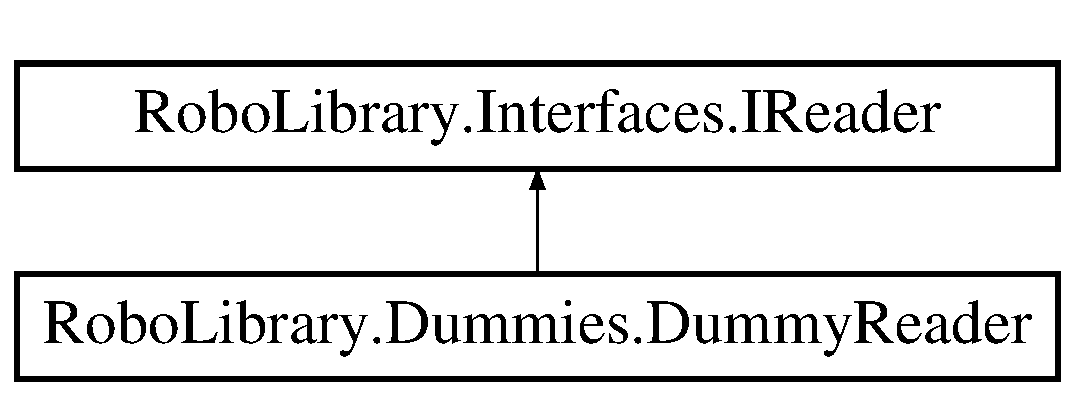
\includegraphics[height=2.000000cm]{class_robo_library_1_1_dummies_1_1_dummy_reader}
\end{center}
\end{figure}
\subsection*{Public Member Functions}
\begin{DoxyCompactItemize}
\item 
\hypertarget{class_robo_library_1_1_dummies_1_1_dummy_reader_ad0dbf81053f910ebf2651df522ab6b0c}{}\label{class_robo_library_1_1_dummies_1_1_dummy_reader_ad0dbf81053f910ebf2651df522ab6b0c} 
void {\bfseries Start\+Listen} (string I\+P\+Adress, Auto\+Reset\+Event are)
\end{DoxyCompactItemize}


The documentation for this class was generated from the following file\+:\begin{DoxyCompactItemize}
\item 
Robo\+Library/\+Dummies/Dummy\+Reader.\+cs\end{DoxyCompactItemize}

\hypertarget{class_robo_library_1_1_dummies_1_1_dummy_u_r10}{}\section{Robo\+Library.\+Dummies.\+Dummy\+U\+R10 Class Reference}
\label{class_robo_library_1_1_dummies_1_1_dummy_u_r10}\index{Robo\+Library.\+Dummies.\+Dummy\+U\+R10@{Robo\+Library.\+Dummies.\+Dummy\+U\+R10}}
\subsection*{Public Attributes}
\begin{DoxyCompactItemize}
\item 
\hypertarget{class_robo_library_1_1_dummies_1_1_dummy_u_r10_a76a637158c69bcf680651946af7b66d8}{}\label{class_robo_library_1_1_dummies_1_1_dummy_u_r10_a76a637158c69bcf680651946af7b66d8} 
\hyperlink{class_robo_library_1_1_u_r_pose}{U\+R\+Pose} {\bfseries pose}
\end{DoxyCompactItemize}
\subsection*{Properties}
\begin{DoxyCompactItemize}
\item 
\hypertarget{class_robo_library_1_1_dummies_1_1_dummy_u_r10_a68900145db5334b73384ab45ede80ba5}{}\label{class_robo_library_1_1_dummies_1_1_dummy_u_r10_a68900145db5334b73384ab45ede80ba5} 
static \hyperlink{class_robo_library_1_1_dummies_1_1_dummy_u_r10}{Dummy\+U\+R10} {\bfseries Instance}\hspace{0.3cm}{\ttfamily  \mbox{[}get\mbox{]}}
\end{DoxyCompactItemize}


The documentation for this class was generated from the following file\+:\begin{DoxyCompactItemize}
\item 
Robo\+Library/\+Dummies/Dummy\+U\+R10.\+cs\end{DoxyCompactItemize}

\hypertarget{class_robo_library_1_1_dummies_1_1_dummy_writer}{}\section{Robo\+Library.\+Dummies.\+Dummy\+Writer Class Reference}
\label{class_robo_library_1_1_dummies_1_1_dummy_writer}\index{Robo\+Library.\+Dummies.\+Dummy\+Writer@{Robo\+Library.\+Dummies.\+Dummy\+Writer}}
Inheritance diagram for Robo\+Library.\+Dummies.\+Dummy\+Writer\+:\begin{figure}[H]
\begin{center}
\leavevmode
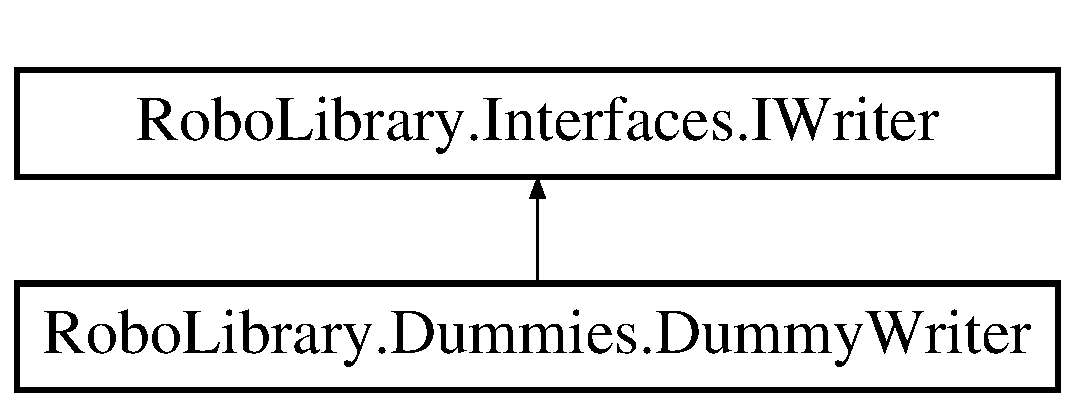
\includegraphics[height=2.000000cm]{class_robo_library_1_1_dummies_1_1_dummy_writer}
\end{center}
\end{figure}
\subsection*{Public Member Functions}
\begin{DoxyCompactItemize}
\item 
\hypertarget{class_robo_library_1_1_dummies_1_1_dummy_writer_a2155b71709d72392aa0ada9242361db2}{}\label{class_robo_library_1_1_dummies_1_1_dummy_writer_a2155b71709d72392aa0ada9242361db2} 
void {\bfseries Add\+U\+R\+Pose} (\hyperlink{class_robo_library_1_1_u_r_pose}{U\+R\+Pose} pose)
\item 
\hypertarget{class_robo_library_1_1_dummies_1_1_dummy_writer_ae57a769174305f42d5c0131b04a20933}{}\label{class_robo_library_1_1_dummies_1_1_dummy_writer_ae57a769174305f42d5c0131b04a20933} 
Configuration\+Data {\bfseries Get\+Configurations} ()
\item 
\hypertarget{class_robo_library_1_1_dummies_1_1_dummy_writer_a39ab96112c6e1bed36372716604cc7d9}{}\label{class_robo_library_1_1_dummies_1_1_dummy_writer_a39ab96112c6e1bed36372716604cc7d9} 
void {\bfseries Send\+Configurations} (Configuration\+Data data)
\item 
\hypertarget{class_robo_library_1_1_dummies_1_1_dummy_writer_a8d9d949161a038abb1d6e75e5879bcc6}{}\label{class_robo_library_1_1_dummies_1_1_dummy_writer_a8d9d949161a038abb1d6e75e5879bcc6} 
void {\bfseries Send\+U\+R\+Pose} (\hyperlink{class_robo_library_1_1_u_r_pose}{U\+R\+Pose} pose)
\end{DoxyCompactItemize}


The documentation for this class was generated from the following file\+:\begin{DoxyCompactItemize}
\item 
Robo\+Library/\+Dummies/Dummy\+Writer.\+cs\end{DoxyCompactItemize}

\hypertarget{interface_robo_library_1_1_interfaces_1_1_i_analyzer}{}\section{Robo\+Library.\+Interfaces.\+I\+Analyzer Interface Reference}
\label{interface_robo_library_1_1_interfaces_1_1_i_analyzer}\index{Robo\+Library.\+Interfaces.\+I\+Analyzer@{Robo\+Library.\+Interfaces.\+I\+Analyzer}}
Inheritance diagram for Robo\+Library.\+Interfaces.\+I\+Analyzer\+:\begin{figure}[H]
\begin{center}
\leavevmode
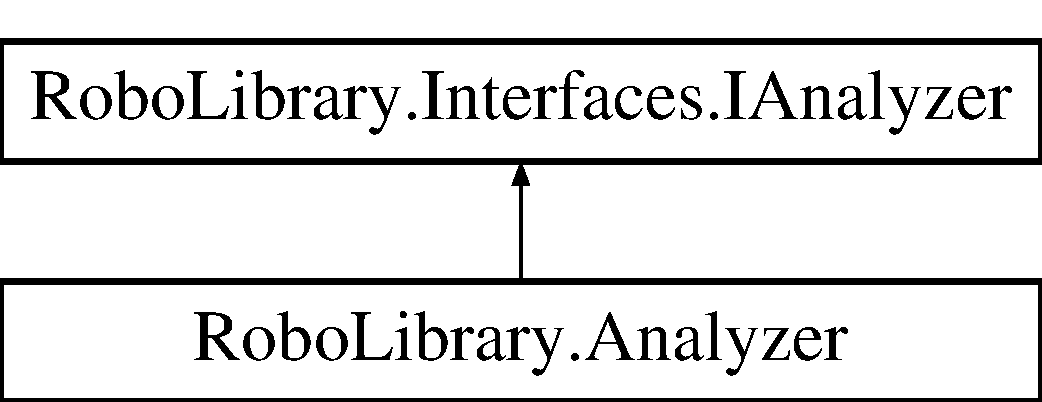
\includegraphics[height=2.000000cm]{interface_robo_library_1_1_interfaces_1_1_i_analyzer}
\end{center}
\end{figure}
\subsection*{Public Member Functions}
\begin{DoxyCompactItemize}
\item 
\hypertarget{interface_robo_library_1_1_interfaces_1_1_i_analyzer_ad1279c13ad39ca2b5fd7002158684910}{}\label{interface_robo_library_1_1_interfaces_1_1_i_analyzer_ad1279c13ad39ca2b5fd7002158684910} 
void {\bfseries Read\+U\+R\+Data} (byte\mbox{[}$\,$\mbox{]} data)
\end{DoxyCompactItemize}


The documentation for this interface was generated from the following file\+:\begin{DoxyCompactItemize}
\item 
Robo\+Library/\+Interfaces/I\+Analyzer.\+cs\end{DoxyCompactItemize}

\hypertarget{interface_robo_library_1_1_interfaces_1_1_i_reader}{}\section{Robo\+Library.\+Interfaces.\+I\+Reader Interface Reference}
\label{interface_robo_library_1_1_interfaces_1_1_i_reader}\index{Robo\+Library.\+Interfaces.\+I\+Reader@{Robo\+Library.\+Interfaces.\+I\+Reader}}
Inheritance diagram for Robo\+Library.\+Interfaces.\+I\+Reader\+:\begin{figure}[H]
\begin{center}
\leavevmode
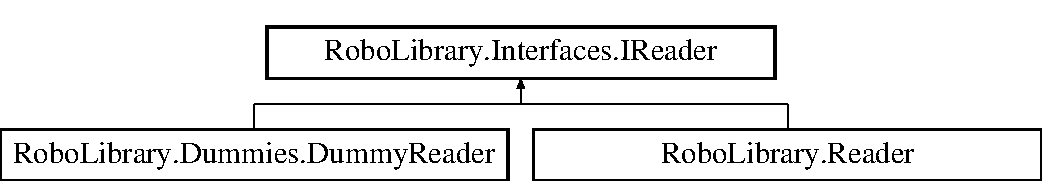
\includegraphics[height=2.000000cm]{interface_robo_library_1_1_interfaces_1_1_i_reader}
\end{center}
\end{figure}
\subsection*{Public Member Functions}
\begin{DoxyCompactItemize}
\item 
\hypertarget{interface_robo_library_1_1_interfaces_1_1_i_reader_a4ce833c4049ed58b8711d5ac55681203}{}\label{interface_robo_library_1_1_interfaces_1_1_i_reader_a4ce833c4049ed58b8711d5ac55681203} 
void {\bfseries Start\+Listen} (string I\+P\+Adress, Auto\+Reset\+Event are)
\end{DoxyCompactItemize}


The documentation for this interface was generated from the following file\+:\begin{DoxyCompactItemize}
\item 
Robo\+Library/\+Interfaces/I\+Reader.\+cs\end{DoxyCompactItemize}

\hypertarget{interface_robo_library_1_1_interfaces_1_1_i_writer}{}\section{Robo\+Library.\+Interfaces.\+I\+Writer Interface Reference}
\label{interface_robo_library_1_1_interfaces_1_1_i_writer}\index{Robo\+Library.\+Interfaces.\+I\+Writer@{Robo\+Library.\+Interfaces.\+I\+Writer}}
Inheritance diagram for Robo\+Library.\+Interfaces.\+I\+Writer\+:\begin{figure}[H]
\begin{center}
\leavevmode
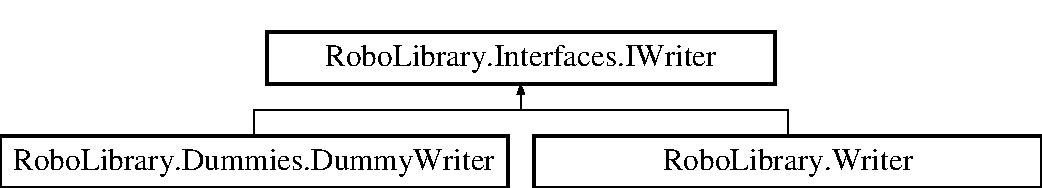
\includegraphics[height=2.000000cm]{interface_robo_library_1_1_interfaces_1_1_i_writer}
\end{center}
\end{figure}
\subsection*{Public Member Functions}
\begin{DoxyCompactItemize}
\item 
\hypertarget{interface_robo_library_1_1_interfaces_1_1_i_writer_a647fab03701336b9231713acd20965c9}{}\label{interface_robo_library_1_1_interfaces_1_1_i_writer_a647fab03701336b9231713acd20965c9} 
void {\bfseries Add\+U\+R\+Pose} (\hyperlink{class_robo_library_1_1_u_r_pose}{U\+R\+Pose} pose)
\item 
\hypertarget{interface_robo_library_1_1_interfaces_1_1_i_writer_a3e88f2733a35867096f26bf636128ed1}{}\label{interface_robo_library_1_1_interfaces_1_1_i_writer_a3e88f2733a35867096f26bf636128ed1} 
void {\bfseries Send\+U\+R\+Pose} (\hyperlink{class_robo_library_1_1_u_r_pose}{U\+R\+Pose} pose)
\item 
\hypertarget{interface_robo_library_1_1_interfaces_1_1_i_writer_a816de14714d3f21cfa3a9b477da24595}{}\label{interface_robo_library_1_1_interfaces_1_1_i_writer_a816de14714d3f21cfa3a9b477da24595} 
Configuration\+Data {\bfseries Get\+Configurations} ()
\item 
\hypertarget{interface_robo_library_1_1_interfaces_1_1_i_writer_adf42668550727c0e9d181925ceb6bc4e}{}\label{interface_robo_library_1_1_interfaces_1_1_i_writer_adf42668550727c0e9d181925ceb6bc4e} 
void {\bfseries Send\+Configurations} (Configuration\+Data data)
\end{DoxyCompactItemize}


The documentation for this interface was generated from the following file\+:\begin{DoxyCompactItemize}
\item 
Robo\+Library/\+Interfaces/I\+Writer.\+cs\end{DoxyCompactItemize}

\hypertarget{class_computer_vision_library_1_1_kinect_fusionizer}{}\section{Computer\+Vision\+Library.\+Kinect\+Fusionizer Class Reference}
\label{class_computer_vision_library_1_1_kinect_fusionizer}\index{Computer\+Vision\+Library.\+Kinect\+Fusionizer@{Computer\+Vision\+Library.\+Kinect\+Fusionizer}}
\subsection*{Public Member Functions}
\begin{DoxyCompactItemize}
\item 
\hypertarget{class_computer_vision_library_1_1_kinect_fusionizer_ad8ec6c5135c56d77d307b59f76d40634}{}\label{class_computer_vision_library_1_1_kinect_fusionizer_ad8ec6c5135c56d77d307b59f76d40634} 
void {\bfseries Set\+Up\+Kinect\+Variables} ()
\end{DoxyCompactItemize}
\subsection*{Public Attributes}
\begin{DoxyCompactItemize}
\item 
\hypertarget{class_computer_vision_library_1_1_kinect_fusionizer_aab0db833b58f1c6f022dcc4a96727621}{}\label{class_computer_vision_library_1_1_kinect_fusionizer_aab0db833b58f1c6f022dcc4a96727621} 
bool {\bfseries Capture\+Current} = false
\item 
\hypertarget{class_computer_vision_library_1_1_kinect_fusionizer_ab7be698214e5029de3ef03a43d492270}{}\label{class_computer_vision_library_1_1_kinect_fusionizer_ab7be698214e5029de3ef03a43d492270} 
Color\+Mesh {\bfseries current\+Mesh}
\end{DoxyCompactItemize}


The documentation for this class was generated from the following file\+:\begin{DoxyCompactItemize}
\item 
Computer\+Vision\+Library/Kinect\+Fusionizer.\+cs\end{DoxyCompactItemize}

\hypertarget{class_robo_library_1_1_logic}{}\section{Robo\+Library.\+Logic Class Reference}
\label{class_robo_library_1_1_logic}\index{Robo\+Library.\+Logic@{Robo\+Library.\+Logic}}
\subsection*{Public Member Functions}
\begin{DoxyCompactItemize}
\item 
\hypertarget{class_robo_library_1_1_logic_a800b2c4e7162b056f8583735a16bc2a9}{}\label{class_robo_library_1_1_logic_a800b2c4e7162b056f8583735a16bc2a9} 
void {\bfseries Send\+Path} ()
\item 
\hypertarget{class_robo_library_1_1_logic_a542ef7edd76d25a6a4db00b64f73d181}{}\label{class_robo_library_1_1_logic_a542ef7edd76d25a6a4db00b64f73d181} 
void {\bfseries Change\+Position\+Rotation} (double x, double y, double z, double rx, double ry, double rz)
\item 
\hypertarget{class_robo_library_1_1_logic_a7cfcf222169cf0a16e6957915207a551}{}\label{class_robo_library_1_1_logic_a7cfcf222169cf0a16e6957915207a551} 
void {\bfseries Send\+Entire\+Pose} (\hyperlink{class_robo_library_1_1_u_r_pose}{U\+R\+Pose} pose)
\end{DoxyCompactItemize}
\subsection*{Properties}
\begin{DoxyCompactItemize}
\item 
\hypertarget{class_robo_library_1_1_logic_a4849fb6b77299570d18ceb82943a4aa7}{}\label{class_robo_library_1_1_logic_a4849fb6b77299570d18ceb82943a4aa7} 
static \hyperlink{class_robo_library_1_1_logic}{Logic} {\bfseries Instance}\hspace{0.3cm}{\ttfamily  \mbox{[}get\mbox{]}}
\end{DoxyCompactItemize}


The documentation for this class was generated from the following file\+:\begin{DoxyCompactItemize}
\item 
Robo\+Library/Logic.\+cs\end{DoxyCompactItemize}

\hypertarget{class_auto_sonography_w_p_f_1_1_main_window}{}\section{Auto\+Sonography\+W\+P\+F.\+Main\+Window Class Reference}
\label{class_auto_sonography_w_p_f_1_1_main_window}\index{Auto\+Sonography\+W\+P\+F.\+Main\+Window@{Auto\+Sonography\+W\+P\+F.\+Main\+Window}}


Interaction logic for Main\+Window.\+xaml  


Inheritance diagram for Auto\+Sonography\+W\+P\+F.\+Main\+Window\+:\begin{figure}[H]
\begin{center}
\leavevmode
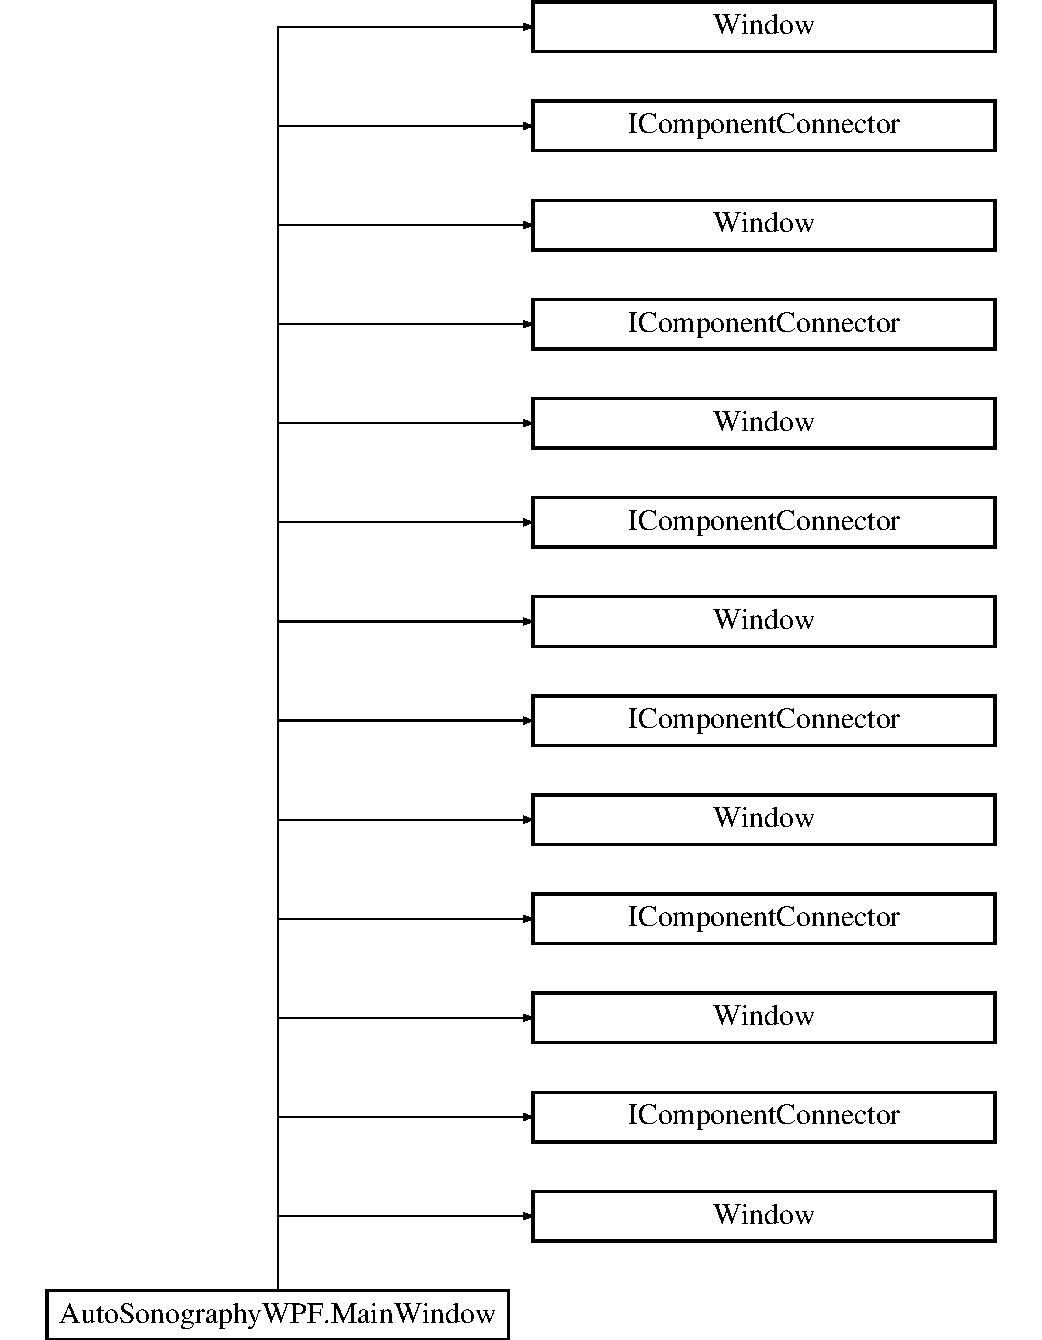
\includegraphics[height=12.000000cm]{class_auto_sonography_w_p_f_1_1_main_window}
\end{center}
\end{figure}
\subsection*{Public Member Functions}
\begin{DoxyCompactItemize}
\item 
void \hyperlink{class_auto_sonography_w_p_f_1_1_main_window_a78046a04c327527f4db402722f7aea35}{Initialize\+Component} ()
\begin{DoxyCompactList}\small\item\em Initialize\+Component \end{DoxyCompactList}\item 
void \hyperlink{class_auto_sonography_w_p_f_1_1_main_window_a78046a04c327527f4db402722f7aea35}{Initialize\+Component} ()
\begin{DoxyCompactList}\small\item\em Initialize\+Component \end{DoxyCompactList}\item 
void \hyperlink{class_auto_sonography_w_p_f_1_1_main_window_a78046a04c327527f4db402722f7aea35}{Initialize\+Component} ()
\begin{DoxyCompactList}\small\item\em Initialize\+Component \end{DoxyCompactList}\item 
void \hyperlink{class_auto_sonography_w_p_f_1_1_main_window_a78046a04c327527f4db402722f7aea35}{Initialize\+Component} ()
\begin{DoxyCompactList}\small\item\em Initialize\+Component \end{DoxyCompactList}\item 
void \hyperlink{class_auto_sonography_w_p_f_1_1_main_window_a78046a04c327527f4db402722f7aea35}{Initialize\+Component} ()
\begin{DoxyCompactList}\small\item\em Initialize\+Component \end{DoxyCompactList}\item 
void \hyperlink{class_auto_sonography_w_p_f_1_1_main_window_a78046a04c327527f4db402722f7aea35}{Initialize\+Component} ()
\begin{DoxyCompactList}\small\item\em Initialize\+Component \end{DoxyCompactList}\end{DoxyCompactItemize}


\subsection{Detailed Description}
Interaction logic for Main\+Window.\+xaml 

\hyperlink{class_auto_sonography_w_p_f_1_1_main_window}{Main\+Window} 

\subsection{Member Function Documentation}
\hypertarget{class_auto_sonography_w_p_f_1_1_main_window_a78046a04c327527f4db402722f7aea35}{}\label{class_auto_sonography_w_p_f_1_1_main_window_a78046a04c327527f4db402722f7aea35} 
\index{Auto\+Sonography\+W\+P\+F\+::\+Main\+Window@{Auto\+Sonography\+W\+P\+F\+::\+Main\+Window}!Initialize\+Component@{Initialize\+Component}}
\index{Initialize\+Component@{Initialize\+Component}!Auto\+Sonography\+W\+P\+F\+::\+Main\+Window@{Auto\+Sonography\+W\+P\+F\+::\+Main\+Window}}
\subsubsection{\texorpdfstring{Initialize\+Component()}{InitializeComponent()}\hspace{0.1cm}{\footnotesize\ttfamily [1/6]}}
{\footnotesize\ttfamily void Auto\+Sonography\+W\+P\+F.\+Main\+Window.\+Initialize\+Component (\begin{DoxyParamCaption}{ }\end{DoxyParamCaption})}



Initialize\+Component 

\hypertarget{class_auto_sonography_w_p_f_1_1_main_window_a78046a04c327527f4db402722f7aea35}{}\label{class_auto_sonography_w_p_f_1_1_main_window_a78046a04c327527f4db402722f7aea35} 
\index{Auto\+Sonography\+W\+P\+F\+::\+Main\+Window@{Auto\+Sonography\+W\+P\+F\+::\+Main\+Window}!Initialize\+Component@{Initialize\+Component}}
\index{Initialize\+Component@{Initialize\+Component}!Auto\+Sonography\+W\+P\+F\+::\+Main\+Window@{Auto\+Sonography\+W\+P\+F\+::\+Main\+Window}}
\subsubsection{\texorpdfstring{Initialize\+Component()}{InitializeComponent()}\hspace{0.1cm}{\footnotesize\ttfamily [2/6]}}
{\footnotesize\ttfamily void Auto\+Sonography\+W\+P\+F.\+Main\+Window.\+Initialize\+Component (\begin{DoxyParamCaption}{ }\end{DoxyParamCaption})}



Initialize\+Component 

\hypertarget{class_auto_sonography_w_p_f_1_1_main_window_a78046a04c327527f4db402722f7aea35}{}\label{class_auto_sonography_w_p_f_1_1_main_window_a78046a04c327527f4db402722f7aea35} 
\index{Auto\+Sonography\+W\+P\+F\+::\+Main\+Window@{Auto\+Sonography\+W\+P\+F\+::\+Main\+Window}!Initialize\+Component@{Initialize\+Component}}
\index{Initialize\+Component@{Initialize\+Component}!Auto\+Sonography\+W\+P\+F\+::\+Main\+Window@{Auto\+Sonography\+W\+P\+F\+::\+Main\+Window}}
\subsubsection{\texorpdfstring{Initialize\+Component()}{InitializeComponent()}\hspace{0.1cm}{\footnotesize\ttfamily [3/6]}}
{\footnotesize\ttfamily void Auto\+Sonography\+W\+P\+F.\+Main\+Window.\+Initialize\+Component (\begin{DoxyParamCaption}{ }\end{DoxyParamCaption})}



Initialize\+Component 

\hypertarget{class_auto_sonography_w_p_f_1_1_main_window_a78046a04c327527f4db402722f7aea35}{}\label{class_auto_sonography_w_p_f_1_1_main_window_a78046a04c327527f4db402722f7aea35} 
\index{Auto\+Sonography\+W\+P\+F\+::\+Main\+Window@{Auto\+Sonography\+W\+P\+F\+::\+Main\+Window}!Initialize\+Component@{Initialize\+Component}}
\index{Initialize\+Component@{Initialize\+Component}!Auto\+Sonography\+W\+P\+F\+::\+Main\+Window@{Auto\+Sonography\+W\+P\+F\+::\+Main\+Window}}
\subsubsection{\texorpdfstring{Initialize\+Component()}{InitializeComponent()}\hspace{0.1cm}{\footnotesize\ttfamily [4/6]}}
{\footnotesize\ttfamily void Auto\+Sonography\+W\+P\+F.\+Main\+Window.\+Initialize\+Component (\begin{DoxyParamCaption}{ }\end{DoxyParamCaption})}



Initialize\+Component 

\hypertarget{class_auto_sonography_w_p_f_1_1_main_window_a78046a04c327527f4db402722f7aea35}{}\label{class_auto_sonography_w_p_f_1_1_main_window_a78046a04c327527f4db402722f7aea35} 
\index{Auto\+Sonography\+W\+P\+F\+::\+Main\+Window@{Auto\+Sonography\+W\+P\+F\+::\+Main\+Window}!Initialize\+Component@{Initialize\+Component}}
\index{Initialize\+Component@{Initialize\+Component}!Auto\+Sonography\+W\+P\+F\+::\+Main\+Window@{Auto\+Sonography\+W\+P\+F\+::\+Main\+Window}}
\subsubsection{\texorpdfstring{Initialize\+Component()}{InitializeComponent()}\hspace{0.1cm}{\footnotesize\ttfamily [5/6]}}
{\footnotesize\ttfamily void Auto\+Sonography\+W\+P\+F.\+Main\+Window.\+Initialize\+Component (\begin{DoxyParamCaption}{ }\end{DoxyParamCaption})}



Initialize\+Component 

\hypertarget{class_auto_sonography_w_p_f_1_1_main_window_a78046a04c327527f4db402722f7aea35}{}\label{class_auto_sonography_w_p_f_1_1_main_window_a78046a04c327527f4db402722f7aea35} 
\index{Auto\+Sonography\+W\+P\+F\+::\+Main\+Window@{Auto\+Sonography\+W\+P\+F\+::\+Main\+Window}!Initialize\+Component@{Initialize\+Component}}
\index{Initialize\+Component@{Initialize\+Component}!Auto\+Sonography\+W\+P\+F\+::\+Main\+Window@{Auto\+Sonography\+W\+P\+F\+::\+Main\+Window}}
\subsubsection{\texorpdfstring{Initialize\+Component()}{InitializeComponent()}\hspace{0.1cm}{\footnotesize\ttfamily [6/6]}}
{\footnotesize\ttfamily void Auto\+Sonography\+W\+P\+F.\+Main\+Window.\+Initialize\+Component (\begin{DoxyParamCaption}{ }\end{DoxyParamCaption})}



Initialize\+Component 



The documentation for this class was generated from the following files\+:\begin{DoxyCompactItemize}
\item 
Auto\+Sonography\+W\+P\+F/Main\+Window.\+xaml.\+cs\item 
Auto\+Sonography\+W\+P\+F/obj/\+Debug/Main\+Window.\+g.\+cs\item 
Auto\+Sonography\+W\+P\+F/obj/\+Debug/Main\+Window.\+g.\+i.\+cs\item 
Auto\+Sonography\+W\+P\+F/obj/\+Debug/Start\+Menu.\+g.\+i.\+cs\end{DoxyCompactItemize}

\hypertarget{class_computer_vision_library_1_1_mesh}{}\section{Computer\+Vision\+Library.\+Mesh Class Reference}
\label{class_computer_vision_library_1_1_mesh}\index{Computer\+Vision\+Library.\+Mesh@{Computer\+Vision\+Library.\+Mesh}}
\subsection*{Static Public Member Functions}
\begin{DoxyCompactItemize}
\item 
\hypertarget{class_computer_vision_library_1_1_mesh_a474e2a8323ace21bf9e9b1a318ec2933}{}\label{class_computer_vision_library_1_1_mesh_a474e2a8323ace21bf9e9b1a318ec2933} 
static \hyperlink{class_computer_vision_library_1_1_mesh}{Mesh} {\bfseries Convert\+To\+Mesh} (Color\+Mesh mesh)
\end{DoxyCompactItemize}
\subsection*{Public Attributes}
\begin{DoxyCompactItemize}
\item 
\hypertarget{class_computer_vision_library_1_1_mesh_a87b64387853c5763cc36162bd240b605}{}\label{class_computer_vision_library_1_1_mesh_a87b64387853c5763cc36162bd240b605} 
List$<$ int $>$ {\bfseries Colors} = new List$<$int$>$()
\item 
\hypertarget{class_computer_vision_library_1_1_mesh_aaceb8d18da9c619358990006cd26463c}{}\label{class_computer_vision_library_1_1_mesh_aaceb8d18da9c619358990006cd26463c} 
List$<$ Vector3 $>$ {\bfseries Normals} = new List$<$Vector3$>$()
\item 
\hypertarget{class_computer_vision_library_1_1_mesh_a8aae428c03c495bef5b794d0906b8d8a}{}\label{class_computer_vision_library_1_1_mesh_a8aae428c03c495bef5b794d0906b8d8a} 
List$<$ int $>$ {\bfseries Triangle\+Indexes} = new List$<$int$>$()
\item 
\hypertarget{class_computer_vision_library_1_1_mesh_a221b5715a75d59ad66df845b95b61825}{}\label{class_computer_vision_library_1_1_mesh_a221b5715a75d59ad66df845b95b61825} 
List$<$ Vector3 $>$ {\bfseries Vertices} = new List$<$Vector3$>$()
\end{DoxyCompactItemize}


The documentation for this class was generated from the following file\+:\begin{DoxyCompactItemize}
\item 
Computer\+Vision\+Library/Color\+Vertex\+Slicer.\+cs\end{DoxyCompactItemize}

\hypertarget{class_robo_library_1_1_mod_bus}{}\section{Robo\+Library.\+Mod\+Bus Class Reference}
\label{class_robo_library_1_1_mod_bus}\index{Robo\+Library.\+Mod\+Bus@{Robo\+Library.\+Mod\+Bus}}


Modbus T\+CP common driver class. This class implements a modbus T\+CP master driver. It supports the following commands\+:  


\subsection*{Public Member Functions}
\begin{DoxyCompactItemize}
\item 
delegate void \hyperlink{class_robo_library_1_1_mod_bus_a497317cafb760023aef4af60fba95c0b}{Response\+Data} (ushort id, byte unit, byte function, byte\mbox{[}$\,$\mbox{]} data)
\begin{DoxyCompactList}\small\item\em Response data event. This event is called when new data arrives\end{DoxyCompactList}\item 
delegate void \hyperlink{class_robo_library_1_1_mod_bus_ac78341a28ded6af9cc33c594315e7c06}{Exception\+Data} (ushort id, byte unit, byte function, byte exception)
\begin{DoxyCompactList}\small\item\em Exception data event. This event is called when the data is incorrect\end{DoxyCompactList}\item 
\hyperlink{class_robo_library_1_1_mod_bus_a060babdf6c052c1b86a160d8ddf68ef1}{Mod\+Bus} ()
\begin{DoxyCompactList}\small\item\em Create master instance without parameters.\end{DoxyCompactList}\item 
\hyperlink{class_robo_library_1_1_mod_bus_a9d7338590ea8f3a27978f7a8e6eebe92}{Mod\+Bus} (string ip, ushort port)
\begin{DoxyCompactList}\small\item\em Create master instance with parameters.\end{DoxyCompactList}\item 
void \hyperlink{class_robo_library_1_1_mod_bus_ac84e8e0281a5b3089742e860cfdd25e5}{Disconnect} ()
\begin{DoxyCompactList}\small\item\em Stop connection to slave.\end{DoxyCompactList}\item 
void \hyperlink{class_robo_library_1_1_mod_bus_ac6c8875d17a35857e67b03d323242477}{Read\+Input\+Register} (ushort id, byte unit, ushort start\+Address, ushort num\+Inputs)
\begin{DoxyCompactList}\small\item\em Read input registers from slave asynchronous. The result is given in the response function.\end{DoxyCompactList}\item 
void \hyperlink{class_robo_library_1_1_mod_bus_ad29bd993efa327748d9929067370bc1a}{Read\+Input\+Register} (ushort id, byte unit, ushort start\+Address, ushort num\+Inputs, ref byte\mbox{[}$\,$\mbox{]} values)
\begin{DoxyCompactList}\small\item\em Read input registers from slave synchronous.\end{DoxyCompactList}\item 
void \hyperlink{class_robo_library_1_1_mod_bus_a0634f07f2e7a02d5a44463eb5f6e7e39}{Write\+Multiple\+Register} (ushort id, byte unit, ushort start\+Address, byte\mbox{[}$\,$\mbox{]} values)
\begin{DoxyCompactList}\small\item\em Write multiple registers in slave asynchronous. The result is given in the response function.\end{DoxyCompactList}\item 
void \hyperlink{class_robo_library_1_1_mod_bus_a205c787f13c0068e875197112552f3a6}{Write\+Multiple\+Register} (ushort id, byte unit, ushort start\+Address, byte\mbox{[}$\,$\mbox{]} values, ref byte\mbox{[}$\,$\mbox{]} result)
\begin{DoxyCompactList}\small\item\em Write multiple registers in slave synchronous.\end{DoxyCompactList}\end{DoxyCompactItemize}
\subsection*{Public Attributes}
\begin{DoxyCompactItemize}
\item 
const byte \hyperlink{class_robo_library_1_1_mod_bus_a7d880ad2a5e4f294d9ce80ab4b201894}{exc\+Illegal\+Function} = 1
\begin{DoxyCompactList}\small\item\em Constant for exception illegal function.\end{DoxyCompactList}\item 
const byte \hyperlink{class_robo_library_1_1_mod_bus_a2b8c0ab4af8f79c7c914116cf96a3753}{exc\+Illegal\+Data\+Adr} = 2
\begin{DoxyCompactList}\small\item\em Constant for exception illegal data address.\end{DoxyCompactList}\item 
const byte \hyperlink{class_robo_library_1_1_mod_bus_a08b557ce75222b5972a6a5b92b6efa99}{exc\+Illegal\+Data\+Val} = 3
\begin{DoxyCompactList}\small\item\em Constant for exception illegal data value.\end{DoxyCompactList}\item 
const byte \hyperlink{class_robo_library_1_1_mod_bus_a23f40b9de42b38035088cf579e960c59}{exc\+Slave\+Device\+Failure} = 4
\begin{DoxyCompactList}\small\item\em Constant for exception slave device failure.\end{DoxyCompactList}\item 
const byte \hyperlink{class_robo_library_1_1_mod_bus_aa8bf5e0ad00a3996ab17afcc1b515ab6}{exc\+Ack} = 5
\begin{DoxyCompactList}\small\item\em Constant for exception acknowledge.\end{DoxyCompactList}\item 
const byte \hyperlink{class_robo_library_1_1_mod_bus_a3057571657af1e777174499c9203aee8}{exc\+Slave\+Is\+Busy} = 6
\begin{DoxyCompactList}\small\item\em Constant for exception slave is busy/booting up.\end{DoxyCompactList}\item 
const byte \hyperlink{class_robo_library_1_1_mod_bus_a94b3937e354438a1e9adc5016c203cfe}{exc\+Gate\+Path\+Unavailable} = 10
\begin{DoxyCompactList}\small\item\em Constant for exception gate path unavailable.\end{DoxyCompactList}\item 
const byte \hyperlink{class_robo_library_1_1_mod_bus_a0c10f797e2ff5ffacb8c8795dd2590bb}{exc\+Exception\+Not\+Connected} = 253
\begin{DoxyCompactList}\small\item\em Constant for exception not connected.\end{DoxyCompactList}\item 
const byte \hyperlink{class_robo_library_1_1_mod_bus_afb92b4598e76f2183460d34fa1c98b2f}{exc\+Exception\+Connection\+Lost} = 254
\begin{DoxyCompactList}\small\item\em Constant for exception connection lost.\end{DoxyCompactList}\item 
const byte \hyperlink{class_robo_library_1_1_mod_bus_a0d3833f9b9c658a3298105f096ee2f28}{exc\+Exception\+Timeout} = 255
\begin{DoxyCompactList}\small\item\em Constant for exception response timeout.\end{DoxyCompactList}\end{DoxyCompactItemize}
\subsection*{Properties}
\begin{DoxyCompactItemize}
\item 
ushort \hyperlink{class_robo_library_1_1_mod_bus_a00b9ec8fc1d37c089ff1e2bee2f7a61a}{timeout}\hspace{0.3cm}{\ttfamily  \mbox{[}get, set\mbox{]}}
\begin{DoxyCompactList}\small\item\em Response timeout. If the slave didn\textquotesingle{}t answers within in this time an exception is called.\end{DoxyCompactList}\item 
ushort \hyperlink{class_robo_library_1_1_mod_bus_a4043bd356bda6e89fd95247956b0708c}{refresh}\hspace{0.3cm}{\ttfamily  \mbox{[}get, set\mbox{]}}
\begin{DoxyCompactList}\small\item\em Refresh timer for slave answer. The class is polling for answer every X ms.\end{DoxyCompactList}\item 
bool \hyperlink{class_robo_library_1_1_mod_bus_ab5a2fb9411e2257f48dd80672326fac1}{connected}\hspace{0.3cm}{\ttfamily  \mbox{[}get\mbox{]}}
\begin{DoxyCompactList}\small\item\em Shows if a connection is active.\end{DoxyCompactList}\end{DoxyCompactItemize}
\subsection*{Events}
\begin{DoxyCompactItemize}
\item 
\hyperlink{class_robo_library_1_1_mod_bus_a497317cafb760023aef4af60fba95c0b}{Response\+Data} \hyperlink{class_robo_library_1_1_mod_bus_a7b2d5617e91faf204d0c8454676353f3}{On\+Response\+Data}
\begin{DoxyCompactList}\small\item\em Response data event. This event is called when new data arrives\end{DoxyCompactList}\item 
\hyperlink{class_robo_library_1_1_mod_bus_ac78341a28ded6af9cc33c594315e7c06}{Exception\+Data} \hyperlink{class_robo_library_1_1_mod_bus_af04afd761811816c0018a8788c33524f}{On\+Exception}
\begin{DoxyCompactList}\small\item\em Exception data event. This event is called when the data is incorrect\end{DoxyCompactList}\end{DoxyCompactItemize}


\subsection{Detailed Description}
Modbus T\+CP common driver class. This class implements a modbus T\+CP master driver. It supports the following commands\+: 

Read coils Read discrete inputs Write single coil Write multiple cooils Read holding register Read input register Write single register Write multiple register

All commands can be sent in synchronous or asynchronous mode. If a value is accessed in synchronous mode the program will stop and wait for slave to response. If the slave didn\textquotesingle{}t answer within a specified time a timeout exception is called. The class uses multi threading for both synchronous and asynchronous access. For the communication two lines are created. This is necessary because the synchronous thread has to wait for a previous command to finish.

\subsection{Constructor \& Destructor Documentation}
\hypertarget{class_robo_library_1_1_mod_bus_a060babdf6c052c1b86a160d8ddf68ef1}{}\label{class_robo_library_1_1_mod_bus_a060babdf6c052c1b86a160d8ddf68ef1} 
\index{Robo\+Library\+::\+Mod\+Bus@{Robo\+Library\+::\+Mod\+Bus}!Mod\+Bus@{Mod\+Bus}}
\index{Mod\+Bus@{Mod\+Bus}!Robo\+Library\+::\+Mod\+Bus@{Robo\+Library\+::\+Mod\+Bus}}
\subsubsection{\texorpdfstring{Mod\+Bus()}{ModBus()}\hspace{0.1cm}{\footnotesize\ttfamily [1/2]}}
{\footnotesize\ttfamily Robo\+Library.\+Mod\+Bus.\+Mod\+Bus (\begin{DoxyParamCaption}{ }\end{DoxyParamCaption})}



Create master instance without parameters.

\hypertarget{class_robo_library_1_1_mod_bus_a9d7338590ea8f3a27978f7a8e6eebe92}{}\label{class_robo_library_1_1_mod_bus_a9d7338590ea8f3a27978f7a8e6eebe92} 
\index{Robo\+Library\+::\+Mod\+Bus@{Robo\+Library\+::\+Mod\+Bus}!Mod\+Bus@{Mod\+Bus}}
\index{Mod\+Bus@{Mod\+Bus}!Robo\+Library\+::\+Mod\+Bus@{Robo\+Library\+::\+Mod\+Bus}}
\subsubsection{\texorpdfstring{Mod\+Bus()}{ModBus()}\hspace{0.1cm}{\footnotesize\ttfamily [2/2]}}
{\footnotesize\ttfamily Robo\+Library.\+Mod\+Bus.\+Mod\+Bus (\begin{DoxyParamCaption}\item[{string}]{ip,  }\item[{ushort}]{port }\end{DoxyParamCaption})}



Create master instance with parameters.


\begin{DoxyParams}{Parameters}
{\em ip} & IP adress of modbus slave.\\
\hline
{\em port} & Port number of modbus slave. Usually port 502 is used.\\
\hline
\end{DoxyParams}


\subsection{Member Function Documentation}
\hypertarget{class_robo_library_1_1_mod_bus_ac84e8e0281a5b3089742e860cfdd25e5}{}\label{class_robo_library_1_1_mod_bus_ac84e8e0281a5b3089742e860cfdd25e5} 
\index{Robo\+Library\+::\+Mod\+Bus@{Robo\+Library\+::\+Mod\+Bus}!Disconnect@{Disconnect}}
\index{Disconnect@{Disconnect}!Robo\+Library\+::\+Mod\+Bus@{Robo\+Library\+::\+Mod\+Bus}}
\subsubsection{\texorpdfstring{Disconnect()}{Disconnect()}}
{\footnotesize\ttfamily void Robo\+Library.\+Mod\+Bus.\+Disconnect (\begin{DoxyParamCaption}{ }\end{DoxyParamCaption})}



Stop connection to slave.

\hypertarget{class_robo_library_1_1_mod_bus_ac78341a28ded6af9cc33c594315e7c06}{}\label{class_robo_library_1_1_mod_bus_ac78341a28ded6af9cc33c594315e7c06} 
\index{Robo\+Library\+::\+Mod\+Bus@{Robo\+Library\+::\+Mod\+Bus}!Exception\+Data@{Exception\+Data}}
\index{Exception\+Data@{Exception\+Data}!Robo\+Library\+::\+Mod\+Bus@{Robo\+Library\+::\+Mod\+Bus}}
\subsubsection{\texorpdfstring{Exception\+Data()}{ExceptionData()}}
{\footnotesize\ttfamily delegate void Robo\+Library.\+Mod\+Bus.\+Exception\+Data (\begin{DoxyParamCaption}\item[{ushort}]{id,  }\item[{byte}]{unit,  }\item[{byte}]{function,  }\item[{byte}]{exception }\end{DoxyParamCaption})}



Exception data event. This event is called when the data is incorrect

\hypertarget{class_robo_library_1_1_mod_bus_ac6c8875d17a35857e67b03d323242477}{}\label{class_robo_library_1_1_mod_bus_ac6c8875d17a35857e67b03d323242477} 
\index{Robo\+Library\+::\+Mod\+Bus@{Robo\+Library\+::\+Mod\+Bus}!Read\+Input\+Register@{Read\+Input\+Register}}
\index{Read\+Input\+Register@{Read\+Input\+Register}!Robo\+Library\+::\+Mod\+Bus@{Robo\+Library\+::\+Mod\+Bus}}
\subsubsection{\texorpdfstring{Read\+Input\+Register()}{ReadInputRegister()}\hspace{0.1cm}{\footnotesize\ttfamily [1/2]}}
{\footnotesize\ttfamily void Robo\+Library.\+Mod\+Bus.\+Read\+Input\+Register (\begin{DoxyParamCaption}\item[{ushort}]{id,  }\item[{byte}]{unit,  }\item[{ushort}]{start\+Address,  }\item[{ushort}]{num\+Inputs }\end{DoxyParamCaption})}



Read input registers from slave asynchronous. The result is given in the response function.


\begin{DoxyParams}{Parameters}
{\em id} & Unique id that marks the transaction. In asynchonous mode this id is given to the callback function.\\
\hline
{\em unit} & Unit identifier (previously slave address). In asynchonous mode this unit is given to the callback function.\\
\hline
{\em start\+Address} & Address from where the data read begins.\\
\hline
{\em num\+Inputs} & Length of data.\\
\hline
\end{DoxyParams}
\hypertarget{class_robo_library_1_1_mod_bus_ad29bd993efa327748d9929067370bc1a}{}\label{class_robo_library_1_1_mod_bus_ad29bd993efa327748d9929067370bc1a} 
\index{Robo\+Library\+::\+Mod\+Bus@{Robo\+Library\+::\+Mod\+Bus}!Read\+Input\+Register@{Read\+Input\+Register}}
\index{Read\+Input\+Register@{Read\+Input\+Register}!Robo\+Library\+::\+Mod\+Bus@{Robo\+Library\+::\+Mod\+Bus}}
\subsubsection{\texorpdfstring{Read\+Input\+Register()}{ReadInputRegister()}\hspace{0.1cm}{\footnotesize\ttfamily [2/2]}}
{\footnotesize\ttfamily void Robo\+Library.\+Mod\+Bus.\+Read\+Input\+Register (\begin{DoxyParamCaption}\item[{ushort}]{id,  }\item[{byte}]{unit,  }\item[{ushort}]{start\+Address,  }\item[{ushort}]{num\+Inputs,  }\item[{ref byte \mbox{[}$\,$\mbox{]}}]{values }\end{DoxyParamCaption})}



Read input registers from slave synchronous.


\begin{DoxyParams}{Parameters}
{\em id} & Unique id that marks the transaction. In asynchonous mode this id is given to the callback function.\\
\hline
{\em unit} & Unit identifier (previously slave address). In asynchonous mode this unit is given to the callback function.\\
\hline
{\em start\+Address} & Address from where the data read begins.\\
\hline
{\em num\+Inputs} & Length of data.\\
\hline
{\em values} & Contains the result of function.\\
\hline
\end{DoxyParams}
\hypertarget{class_robo_library_1_1_mod_bus_a497317cafb760023aef4af60fba95c0b}{}\label{class_robo_library_1_1_mod_bus_a497317cafb760023aef4af60fba95c0b} 
\index{Robo\+Library\+::\+Mod\+Bus@{Robo\+Library\+::\+Mod\+Bus}!Response\+Data@{Response\+Data}}
\index{Response\+Data@{Response\+Data}!Robo\+Library\+::\+Mod\+Bus@{Robo\+Library\+::\+Mod\+Bus}}
\subsubsection{\texorpdfstring{Response\+Data()}{ResponseData()}}
{\footnotesize\ttfamily delegate void Robo\+Library.\+Mod\+Bus.\+Response\+Data (\begin{DoxyParamCaption}\item[{ushort}]{id,  }\item[{byte}]{unit,  }\item[{byte}]{function,  }\item[{byte \mbox{[}$\,$\mbox{]}}]{data }\end{DoxyParamCaption})}



Response data event. This event is called when new data arrives

\hypertarget{class_robo_library_1_1_mod_bus_a0634f07f2e7a02d5a44463eb5f6e7e39}{}\label{class_robo_library_1_1_mod_bus_a0634f07f2e7a02d5a44463eb5f6e7e39} 
\index{Robo\+Library\+::\+Mod\+Bus@{Robo\+Library\+::\+Mod\+Bus}!Write\+Multiple\+Register@{Write\+Multiple\+Register}}
\index{Write\+Multiple\+Register@{Write\+Multiple\+Register}!Robo\+Library\+::\+Mod\+Bus@{Robo\+Library\+::\+Mod\+Bus}}
\subsubsection{\texorpdfstring{Write\+Multiple\+Register()}{WriteMultipleRegister()}\hspace{0.1cm}{\footnotesize\ttfamily [1/2]}}
{\footnotesize\ttfamily void Robo\+Library.\+Mod\+Bus.\+Write\+Multiple\+Register (\begin{DoxyParamCaption}\item[{ushort}]{id,  }\item[{byte}]{unit,  }\item[{ushort}]{start\+Address,  }\item[{byte \mbox{[}$\,$\mbox{]}}]{values }\end{DoxyParamCaption})}



Write multiple registers in slave asynchronous. The result is given in the response function.


\begin{DoxyParams}{Parameters}
{\em id} & Unique id that marks the transaction. In asynchonous mode this id is given to the callback function.\\
\hline
{\em unit} & Unit identifier (previously slave address). In asynchonous mode this unit is given to the callback function.\\
\hline
{\em start\+Address} & Address to where the data is written.\\
\hline
{\em values} & Contains the register information.\\
\hline
\end{DoxyParams}
\hypertarget{class_robo_library_1_1_mod_bus_a205c787f13c0068e875197112552f3a6}{}\label{class_robo_library_1_1_mod_bus_a205c787f13c0068e875197112552f3a6} 
\index{Robo\+Library\+::\+Mod\+Bus@{Robo\+Library\+::\+Mod\+Bus}!Write\+Multiple\+Register@{Write\+Multiple\+Register}}
\index{Write\+Multiple\+Register@{Write\+Multiple\+Register}!Robo\+Library\+::\+Mod\+Bus@{Robo\+Library\+::\+Mod\+Bus}}
\subsubsection{\texorpdfstring{Write\+Multiple\+Register()}{WriteMultipleRegister()}\hspace{0.1cm}{\footnotesize\ttfamily [2/2]}}
{\footnotesize\ttfamily void Robo\+Library.\+Mod\+Bus.\+Write\+Multiple\+Register (\begin{DoxyParamCaption}\item[{ushort}]{id,  }\item[{byte}]{unit,  }\item[{ushort}]{start\+Address,  }\item[{byte \mbox{[}$\,$\mbox{]}}]{values,  }\item[{ref byte \mbox{[}$\,$\mbox{]}}]{result }\end{DoxyParamCaption})}



Write multiple registers in slave synchronous.


\begin{DoxyParams}{Parameters}
{\em id} & Unique id that marks the transaction. In asynchonous mode this id is given to the callback function.\\
\hline
{\em unit} & Unit identifier (previously slave address). In asynchonous mode this unit is given to the callback function.\\
\hline
{\em start\+Address} & Address to where the data is written.\\
\hline
{\em values} & Contains the register information.\\
\hline
{\em result} & Contains the result of the synchronous write.\\
\hline
\end{DoxyParams}


\subsection{Member Data Documentation}
\hypertarget{class_robo_library_1_1_mod_bus_aa8bf5e0ad00a3996ab17afcc1b515ab6}{}\label{class_robo_library_1_1_mod_bus_aa8bf5e0ad00a3996ab17afcc1b515ab6} 
\index{Robo\+Library\+::\+Mod\+Bus@{Robo\+Library\+::\+Mod\+Bus}!exc\+Ack@{exc\+Ack}}
\index{exc\+Ack@{exc\+Ack}!Robo\+Library\+::\+Mod\+Bus@{Robo\+Library\+::\+Mod\+Bus}}
\subsubsection{\texorpdfstring{exc\+Ack}{excAck}}
{\footnotesize\ttfamily const byte Robo\+Library.\+Mod\+Bus.\+exc\+Ack = 5}



Constant for exception acknowledge.

\hypertarget{class_robo_library_1_1_mod_bus_afb92b4598e76f2183460d34fa1c98b2f}{}\label{class_robo_library_1_1_mod_bus_afb92b4598e76f2183460d34fa1c98b2f} 
\index{Robo\+Library\+::\+Mod\+Bus@{Robo\+Library\+::\+Mod\+Bus}!exc\+Exception\+Connection\+Lost@{exc\+Exception\+Connection\+Lost}}
\index{exc\+Exception\+Connection\+Lost@{exc\+Exception\+Connection\+Lost}!Robo\+Library\+::\+Mod\+Bus@{Robo\+Library\+::\+Mod\+Bus}}
\subsubsection{\texorpdfstring{exc\+Exception\+Connection\+Lost}{excExceptionConnectionLost}}
{\footnotesize\ttfamily const byte Robo\+Library.\+Mod\+Bus.\+exc\+Exception\+Connection\+Lost = 254}



Constant for exception connection lost.

\hypertarget{class_robo_library_1_1_mod_bus_a0c10f797e2ff5ffacb8c8795dd2590bb}{}\label{class_robo_library_1_1_mod_bus_a0c10f797e2ff5ffacb8c8795dd2590bb} 
\index{Robo\+Library\+::\+Mod\+Bus@{Robo\+Library\+::\+Mod\+Bus}!exc\+Exception\+Not\+Connected@{exc\+Exception\+Not\+Connected}}
\index{exc\+Exception\+Not\+Connected@{exc\+Exception\+Not\+Connected}!Robo\+Library\+::\+Mod\+Bus@{Robo\+Library\+::\+Mod\+Bus}}
\subsubsection{\texorpdfstring{exc\+Exception\+Not\+Connected}{excExceptionNotConnected}}
{\footnotesize\ttfamily const byte Robo\+Library.\+Mod\+Bus.\+exc\+Exception\+Not\+Connected = 253}



Constant for exception not connected.

\hypertarget{class_robo_library_1_1_mod_bus_a0d3833f9b9c658a3298105f096ee2f28}{}\label{class_robo_library_1_1_mod_bus_a0d3833f9b9c658a3298105f096ee2f28} 
\index{Robo\+Library\+::\+Mod\+Bus@{Robo\+Library\+::\+Mod\+Bus}!exc\+Exception\+Timeout@{exc\+Exception\+Timeout}}
\index{exc\+Exception\+Timeout@{exc\+Exception\+Timeout}!Robo\+Library\+::\+Mod\+Bus@{Robo\+Library\+::\+Mod\+Bus}}
\subsubsection{\texorpdfstring{exc\+Exception\+Timeout}{excExceptionTimeout}}
{\footnotesize\ttfamily const byte Robo\+Library.\+Mod\+Bus.\+exc\+Exception\+Timeout = 255}



Constant for exception response timeout.

\hypertarget{class_robo_library_1_1_mod_bus_a94b3937e354438a1e9adc5016c203cfe}{}\label{class_robo_library_1_1_mod_bus_a94b3937e354438a1e9adc5016c203cfe} 
\index{Robo\+Library\+::\+Mod\+Bus@{Robo\+Library\+::\+Mod\+Bus}!exc\+Gate\+Path\+Unavailable@{exc\+Gate\+Path\+Unavailable}}
\index{exc\+Gate\+Path\+Unavailable@{exc\+Gate\+Path\+Unavailable}!Robo\+Library\+::\+Mod\+Bus@{Robo\+Library\+::\+Mod\+Bus}}
\subsubsection{\texorpdfstring{exc\+Gate\+Path\+Unavailable}{excGatePathUnavailable}}
{\footnotesize\ttfamily const byte Robo\+Library.\+Mod\+Bus.\+exc\+Gate\+Path\+Unavailable = 10}



Constant for exception gate path unavailable.

\hypertarget{class_robo_library_1_1_mod_bus_a2b8c0ab4af8f79c7c914116cf96a3753}{}\label{class_robo_library_1_1_mod_bus_a2b8c0ab4af8f79c7c914116cf96a3753} 
\index{Robo\+Library\+::\+Mod\+Bus@{Robo\+Library\+::\+Mod\+Bus}!exc\+Illegal\+Data\+Adr@{exc\+Illegal\+Data\+Adr}}
\index{exc\+Illegal\+Data\+Adr@{exc\+Illegal\+Data\+Adr}!Robo\+Library\+::\+Mod\+Bus@{Robo\+Library\+::\+Mod\+Bus}}
\subsubsection{\texorpdfstring{exc\+Illegal\+Data\+Adr}{excIllegalDataAdr}}
{\footnotesize\ttfamily const byte Robo\+Library.\+Mod\+Bus.\+exc\+Illegal\+Data\+Adr = 2}



Constant for exception illegal data address.

\hypertarget{class_robo_library_1_1_mod_bus_a08b557ce75222b5972a6a5b92b6efa99}{}\label{class_robo_library_1_1_mod_bus_a08b557ce75222b5972a6a5b92b6efa99} 
\index{Robo\+Library\+::\+Mod\+Bus@{Robo\+Library\+::\+Mod\+Bus}!exc\+Illegal\+Data\+Val@{exc\+Illegal\+Data\+Val}}
\index{exc\+Illegal\+Data\+Val@{exc\+Illegal\+Data\+Val}!Robo\+Library\+::\+Mod\+Bus@{Robo\+Library\+::\+Mod\+Bus}}
\subsubsection{\texorpdfstring{exc\+Illegal\+Data\+Val}{excIllegalDataVal}}
{\footnotesize\ttfamily const byte Robo\+Library.\+Mod\+Bus.\+exc\+Illegal\+Data\+Val = 3}



Constant for exception illegal data value.

\hypertarget{class_robo_library_1_1_mod_bus_a7d880ad2a5e4f294d9ce80ab4b201894}{}\label{class_robo_library_1_1_mod_bus_a7d880ad2a5e4f294d9ce80ab4b201894} 
\index{Robo\+Library\+::\+Mod\+Bus@{Robo\+Library\+::\+Mod\+Bus}!exc\+Illegal\+Function@{exc\+Illegal\+Function}}
\index{exc\+Illegal\+Function@{exc\+Illegal\+Function}!Robo\+Library\+::\+Mod\+Bus@{Robo\+Library\+::\+Mod\+Bus}}
\subsubsection{\texorpdfstring{exc\+Illegal\+Function}{excIllegalFunction}}
{\footnotesize\ttfamily const byte Robo\+Library.\+Mod\+Bus.\+exc\+Illegal\+Function = 1}



Constant for exception illegal function.

\hypertarget{class_robo_library_1_1_mod_bus_a23f40b9de42b38035088cf579e960c59}{}\label{class_robo_library_1_1_mod_bus_a23f40b9de42b38035088cf579e960c59} 
\index{Robo\+Library\+::\+Mod\+Bus@{Robo\+Library\+::\+Mod\+Bus}!exc\+Slave\+Device\+Failure@{exc\+Slave\+Device\+Failure}}
\index{exc\+Slave\+Device\+Failure@{exc\+Slave\+Device\+Failure}!Robo\+Library\+::\+Mod\+Bus@{Robo\+Library\+::\+Mod\+Bus}}
\subsubsection{\texorpdfstring{exc\+Slave\+Device\+Failure}{excSlaveDeviceFailure}}
{\footnotesize\ttfamily const byte Robo\+Library.\+Mod\+Bus.\+exc\+Slave\+Device\+Failure = 4}



Constant for exception slave device failure.

\hypertarget{class_robo_library_1_1_mod_bus_a3057571657af1e777174499c9203aee8}{}\label{class_robo_library_1_1_mod_bus_a3057571657af1e777174499c9203aee8} 
\index{Robo\+Library\+::\+Mod\+Bus@{Robo\+Library\+::\+Mod\+Bus}!exc\+Slave\+Is\+Busy@{exc\+Slave\+Is\+Busy}}
\index{exc\+Slave\+Is\+Busy@{exc\+Slave\+Is\+Busy}!Robo\+Library\+::\+Mod\+Bus@{Robo\+Library\+::\+Mod\+Bus}}
\subsubsection{\texorpdfstring{exc\+Slave\+Is\+Busy}{excSlaveIsBusy}}
{\footnotesize\ttfamily const byte Robo\+Library.\+Mod\+Bus.\+exc\+Slave\+Is\+Busy = 6}



Constant for exception slave is busy/booting up.



\subsection{Property Documentation}
\hypertarget{class_robo_library_1_1_mod_bus_ab5a2fb9411e2257f48dd80672326fac1}{}\label{class_robo_library_1_1_mod_bus_ab5a2fb9411e2257f48dd80672326fac1} 
\index{Robo\+Library\+::\+Mod\+Bus@{Robo\+Library\+::\+Mod\+Bus}!connected@{connected}}
\index{connected@{connected}!Robo\+Library\+::\+Mod\+Bus@{Robo\+Library\+::\+Mod\+Bus}}
\subsubsection{\texorpdfstring{connected}{connected}}
{\footnotesize\ttfamily bool Robo\+Library.\+Mod\+Bus.\+connected\hspace{0.3cm}{\ttfamily [get]}}



Shows if a connection is active.

\hypertarget{class_robo_library_1_1_mod_bus_a4043bd356bda6e89fd95247956b0708c}{}\label{class_robo_library_1_1_mod_bus_a4043bd356bda6e89fd95247956b0708c} 
\index{Robo\+Library\+::\+Mod\+Bus@{Robo\+Library\+::\+Mod\+Bus}!refresh@{refresh}}
\index{refresh@{refresh}!Robo\+Library\+::\+Mod\+Bus@{Robo\+Library\+::\+Mod\+Bus}}
\subsubsection{\texorpdfstring{refresh}{refresh}}
{\footnotesize\ttfamily ushort Robo\+Library.\+Mod\+Bus.\+refresh\hspace{0.3cm}{\ttfamily [get]}, {\ttfamily [set]}}



Refresh timer for slave answer. The class is polling for answer every X ms.

The default value is 10ms.\hypertarget{class_robo_library_1_1_mod_bus_a00b9ec8fc1d37c089ff1e2bee2f7a61a}{}\label{class_robo_library_1_1_mod_bus_a00b9ec8fc1d37c089ff1e2bee2f7a61a} 
\index{Robo\+Library\+::\+Mod\+Bus@{Robo\+Library\+::\+Mod\+Bus}!timeout@{timeout}}
\index{timeout@{timeout}!Robo\+Library\+::\+Mod\+Bus@{Robo\+Library\+::\+Mod\+Bus}}
\subsubsection{\texorpdfstring{timeout}{timeout}}
{\footnotesize\ttfamily ushort Robo\+Library.\+Mod\+Bus.\+timeout\hspace{0.3cm}{\ttfamily [get]}, {\ttfamily [set]}}



Response timeout. If the slave didn\textquotesingle{}t answers within in this time an exception is called.

The default value is 500ms.

\subsection{Event Documentation}
\hypertarget{class_robo_library_1_1_mod_bus_af04afd761811816c0018a8788c33524f}{}\label{class_robo_library_1_1_mod_bus_af04afd761811816c0018a8788c33524f} 
\index{Robo\+Library\+::\+Mod\+Bus@{Robo\+Library\+::\+Mod\+Bus}!On\+Exception@{On\+Exception}}
\index{On\+Exception@{On\+Exception}!Robo\+Library\+::\+Mod\+Bus@{Robo\+Library\+::\+Mod\+Bus}}
\subsubsection{\texorpdfstring{On\+Exception}{OnException}}
{\footnotesize\ttfamily \hyperlink{class_robo_library_1_1_mod_bus_ac78341a28ded6af9cc33c594315e7c06}{Exception\+Data} Robo\+Library.\+Mod\+Bus.\+On\+Exception}



Exception data event. This event is called when the data is incorrect

\hypertarget{class_robo_library_1_1_mod_bus_a7b2d5617e91faf204d0c8454676353f3}{}\label{class_robo_library_1_1_mod_bus_a7b2d5617e91faf204d0c8454676353f3} 
\index{Robo\+Library\+::\+Mod\+Bus@{Robo\+Library\+::\+Mod\+Bus}!On\+Response\+Data@{On\+Response\+Data}}
\index{On\+Response\+Data@{On\+Response\+Data}!Robo\+Library\+::\+Mod\+Bus@{Robo\+Library\+::\+Mod\+Bus}}
\subsubsection{\texorpdfstring{On\+Response\+Data}{OnResponseData}}
{\footnotesize\ttfamily \hyperlink{class_robo_library_1_1_mod_bus_a497317cafb760023aef4af60fba95c0b}{Response\+Data} Robo\+Library.\+Mod\+Bus.\+On\+Response\+Data}



Response data event. This event is called when new data arrives



The documentation for this class was generated from the following file\+:\begin{DoxyCompactItemize}
\item 
Robo\+Library/Mod\+Bus.\+cs\end{DoxyCompactItemize}

\hypertarget{class_robo_library_1_1_path_creator}{}\section{Robo\+Library.\+Path\+Creator Class Reference}
\label{class_robo_library_1_1_path_creator}\index{Robo\+Library.\+Path\+Creator@{Robo\+Library.\+Path\+Creator}}
\subsection*{Public Member Functions}
\begin{DoxyCompactItemize}
\item 
\hypertarget{class_robo_library_1_1_path_creator_a4d9db7f14e09ff2cf263cbfd4120dd19}{}\label{class_robo_library_1_1_path_creator_a4d9db7f14e09ff2cf263cbfd4120dd19} 
List$<$ \hyperlink{class_robo_library_1_1_u_r_pose}{U\+R\+Pose} $>$ {\bfseries Return\+Two\+Test\+Points} (\hyperlink{class_robo_library_1_1_u_r_pose}{U\+R\+Pose} current\+Pose)
\item 
\hypertarget{class_robo_library_1_1_path_creator_a1e98e0454508db507fdc4552bc8b26c7}{}\label{class_robo_library_1_1_path_creator_a1e98e0454508db507fdc4552bc8b26c7} 
List$<$ \hyperlink{class_robo_library_1_1_u_r_pose}{U\+R\+Pose} $>$ {\bfseries Return\+Circle} ()
\item 
\hypertarget{class_robo_library_1_1_path_creator_ad16f16cc4a694df8cb142eb71b48a60c}{}\label{class_robo_library_1_1_path_creator_ad16f16cc4a694df8cb142eb71b48a60c} 
List$<$ \hyperlink{class_robo_library_1_1_u_r_pose}{U\+R\+Pose} $>$ {\bfseries generate\+\_\+circle} ()
\end{DoxyCompactItemize}


The documentation for this class was generated from the following file\+:\begin{DoxyCompactItemize}
\item 
Robo\+Library/Path\+Creator.\+cs\end{DoxyCompactItemize}

\hypertarget{class_robo_library_1_1_path_feeder}{}\section{Robo\+Library.\+Path\+Feeder Class Reference}
\label{class_robo_library_1_1_path_feeder}\index{Robo\+Library.\+Path\+Feeder@{Robo\+Library.\+Path\+Feeder}}
\subsection*{Public Member Functions}
\begin{DoxyCompactItemize}
\item 
\hypertarget{class_robo_library_1_1_path_feeder_a13726d814ab88a8950e2d2aca56e39cd}{}\label{class_robo_library_1_1_path_feeder_a13726d814ab88a8950e2d2aca56e39cd} 
void {\bfseries Run\+Path} (List$<$ \hyperlink{class_robo_library_1_1_u_r_pose}{U\+R\+Pose} $>$ path)
\item 
\hypertarget{class_robo_library_1_1_path_feeder_a0a6035a947d529023748323ffc383f4d}{}\label{class_robo_library_1_1_path_feeder_a0a6035a947d529023748323ffc383f4d} 
bool {\bfseries Is\+Close\+Enough} (\hyperlink{class_robo_library_1_1_u_r_pose}{U\+R\+Pose} target, \hyperlink{class_robo_library_1_1_u_r_pose}{U\+R\+Pose} actual)
\end{DoxyCompactItemize}
\subsection*{Public Attributes}
\begin{DoxyCompactItemize}
\item 
\hypertarget{class_robo_library_1_1_path_feeder_a0b00d377406135530dd4f8db06b1af35}{}\label{class_robo_library_1_1_path_feeder_a0b00d377406135530dd4f8db06b1af35} 
bool {\bfseries Running\+Path}
\item 
\hypertarget{class_robo_library_1_1_path_feeder_aa173e29e43684b244bb098781f69e381}{}\label{class_robo_library_1_1_path_feeder_aa173e29e43684b244bb098781f69e381} 
bool {\bfseries Should\+Run} = true
\end{DoxyCompactItemize}
\subsection*{Static Public Attributes}
\begin{DoxyCompactItemize}
\item 
\hypertarget{class_robo_library_1_1_path_feeder_a7594eb7457b5143effd224d78e650750}{}\label{class_robo_library_1_1_path_feeder_a7594eb7457b5143effd224d78e650750} 
static double {\bfseries minimum\+\_\+proximity\+\_\+position} = 0.\+01d
\item 
\hypertarget{class_robo_library_1_1_path_feeder_ac0882a60619c474f9cbf67f0bf094725}{}\label{class_robo_library_1_1_path_feeder_ac0882a60619c474f9cbf67f0bf094725} 
static double {\bfseries minimum\+\_\+proximity\+\_\+rotation} = 1
\end{DoxyCompactItemize}


The documentation for this class was generated from the following file\+:\begin{DoxyCompactItemize}
\item 
Robo\+Library/Path\+Feeder.\+cs\end{DoxyCompactItemize}

\hypertarget{class_computer_vision_library_1_1_p_l_y_exporter}{}\section{Computer\+Vision\+Library.\+P\+L\+Y\+Exporter Class Reference}
\label{class_computer_vision_library_1_1_p_l_y_exporter}\index{Computer\+Vision\+Library.\+P\+L\+Y\+Exporter@{Computer\+Vision\+Library.\+P\+L\+Y\+Exporter}}
\subsection*{Static Public Member Functions}
\begin{DoxyCompactItemize}
\item 
\hypertarget{class_computer_vision_library_1_1_p_l_y_exporter_a061c4bc25d99cd1fe5eb47398ef05eec}{}\label{class_computer_vision_library_1_1_p_l_y_exporter_a061c4bc25d99cd1fe5eb47398ef05eec} 
static bool {\bfseries Output} (Color\+Mesh mesh, ref string location)
\item 
\hypertarget{class_computer_vision_library_1_1_p_l_y_exporter_aa43bff677fa9b8374fa48dd69a7c7da6}{}\label{class_computer_vision_library_1_1_p_l_y_exporter_aa43bff677fa9b8374fa48dd69a7c7da6} 
static bool {\bfseries Output} (\hyperlink{class_computer_vision_library_1_1_mesh}{Mesh} mesh, ref string location)
\end{DoxyCompactItemize}


The documentation for this class was generated from the following file\+:\begin{DoxyCompactItemize}
\item 
Computer\+Vision\+Library/P\+L\+Y\+Exporter.\+cs\end{DoxyCompactItemize}

\hypertarget{class_robo_library_1_1_reader}{}\section{Robo\+Library.\+Reader Class Reference}
\label{class_robo_library_1_1_reader}\index{Robo\+Library.\+Reader@{Robo\+Library.\+Reader}}
Inheritance diagram for Robo\+Library.\+Reader\+:\begin{figure}[H]
\begin{center}
\leavevmode
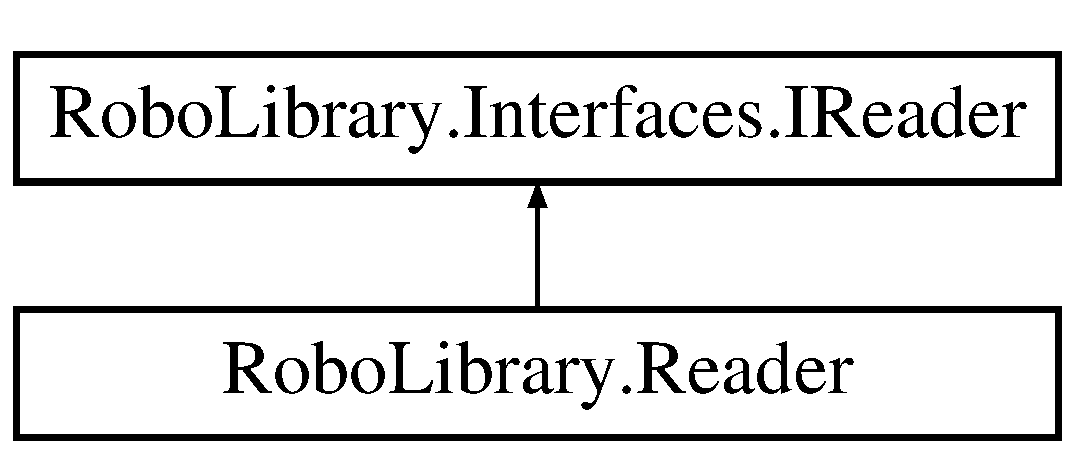
\includegraphics[height=2.000000cm]{class_robo_library_1_1_reader}
\end{center}
\end{figure}
\subsection*{Public Member Functions}
\begin{DoxyCompactItemize}
\item 
\hypertarget{class_robo_library_1_1_reader_a9c0b25d0958e6d6a59c3bf9f772d37d0}{}\label{class_robo_library_1_1_reader_a9c0b25d0958e6d6a59c3bf9f772d37d0} 
void {\bfseries Start\+Listen} (string ip\+\_\+address, Auto\+Reset\+Event are)
\item 
\hypertarget{class_robo_library_1_1_reader_adf6670473fb8dbc1cafbd82dbfae3c56}{}\label{class_robo_library_1_1_reader_adf6670473fb8dbc1cafbd82dbfae3c56} 
void {\bfseries Request\+Socket\+Shutdown} ()
\end{DoxyCompactItemize}
\subsection*{Public Attributes}
\begin{DoxyCompactItemize}
\item 
\hypertarget{class_robo_library_1_1_reader_a930d627919a5268586350aa9b61e5f2b}{}\label{class_robo_library_1_1_reader_a930d627919a5268586350aa9b61e5f2b} 
bool {\bfseries Is\+Connected} = false
\item 
\hypertarget{class_robo_library_1_1_reader_a2c4d988beace95d044f038085993bc82}{}\label{class_robo_library_1_1_reader_a2c4d988beace95d044f038085993bc82} 
bool {\bfseries Should\+Stop} = false
\end{DoxyCompactItemize}


The documentation for this class was generated from the following file\+:\begin{DoxyCompactItemize}
\item 
Robo\+Library/Reader.\+cs\end{DoxyCompactItemize}

\hypertarget{class_robo_library_1_1_robo_master}{}\section{Robo\+Library.\+Robo\+Master Class Reference}
\label{class_robo_library_1_1_robo_master}\index{Robo\+Library.\+Robo\+Master@{Robo\+Library.\+Robo\+Master}}


The documentation for this class was generated from the following file\+:\begin{DoxyCompactItemize}
\item 
Robo\+Library/Robo\+Master.\+cs\end{DoxyCompactItemize}

\hypertarget{class_robo_library_1_1_testing_extensions_1_1_shape_generator}{}\section{Robo\+Library.\+Testing\+Extensions.\+Shape\+Generator Class Reference}
\label{class_robo_library_1_1_testing_extensions_1_1_shape_generator}\index{Robo\+Library.\+Testing\+Extensions.\+Shape\+Generator@{Robo\+Library.\+Testing\+Extensions.\+Shape\+Generator}}


The documentation for this class was generated from the following file\+:\begin{DoxyCompactItemize}
\item 
Robo\+Library/\+Testing\+Extensions/Shape\+Generator.\+cs\end{DoxyCompactItemize}

\hypertarget{class_auto_sonography_w_p_f_1_1_ultrasound_scan_menu}{}\section{Auto\+Sonography\+W\+P\+F.\+Ultrasound\+Scan\+Menu Class Reference}
\label{class_auto_sonography_w_p_f_1_1_ultrasound_scan_menu}\index{Auto\+Sonography\+W\+P\+F.\+Ultrasound\+Scan\+Menu@{Auto\+Sonography\+W\+P\+F.\+Ultrasound\+Scan\+Menu}}


\hyperlink{class_auto_sonography_w_p_f_1_1_ultrasound_scan_menu}{Ultrasound\+Scan\+Menu}  


Inheritance diagram for Auto\+Sonography\+W\+P\+F.\+Ultrasound\+Scan\+Menu\+:\begin{figure}[H]
\begin{center}
\leavevmode
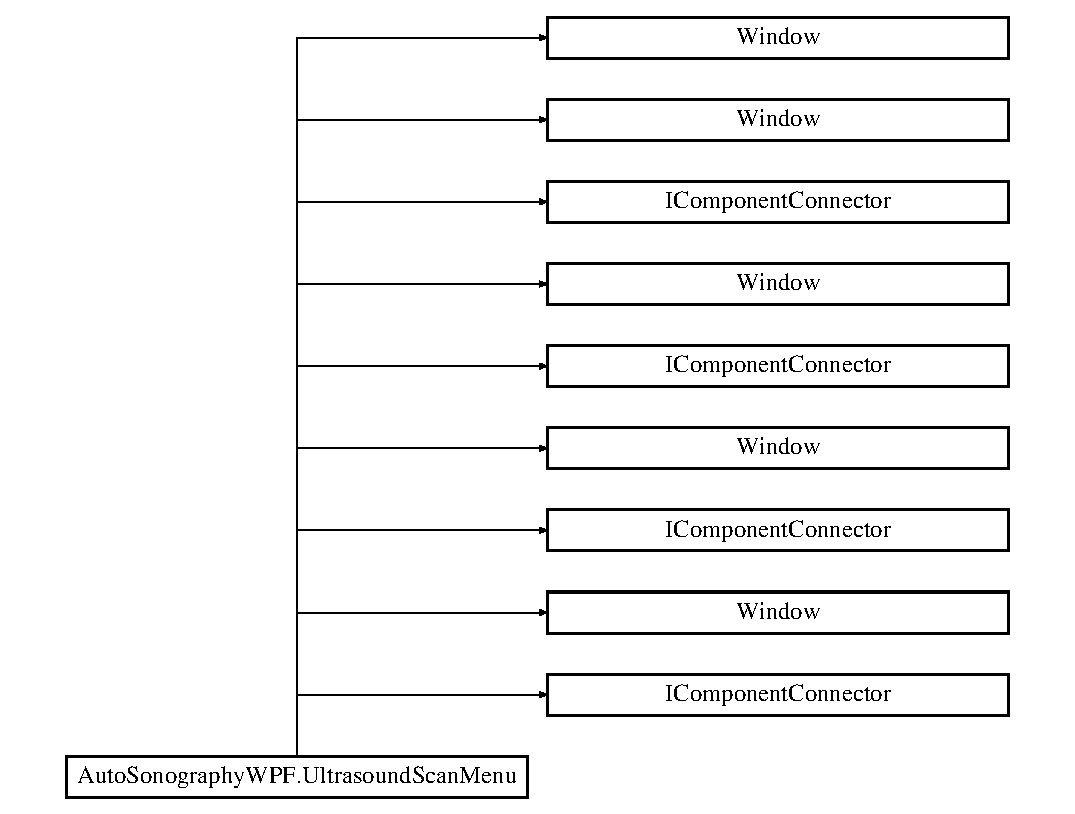
\includegraphics[height=10.000000cm]{class_auto_sonography_w_p_f_1_1_ultrasound_scan_menu}
\end{center}
\end{figure}
\subsection*{Public Member Functions}
\begin{DoxyCompactItemize}
\item 
void \hyperlink{class_auto_sonography_w_p_f_1_1_ultrasound_scan_menu_a16a3c05a908d3edf244d0e5ec887519b}{Initialize\+Component} ()
\begin{DoxyCompactList}\small\item\em Initialize\+Component \end{DoxyCompactList}\item 
void \hyperlink{class_auto_sonography_w_p_f_1_1_ultrasound_scan_menu_a16a3c05a908d3edf244d0e5ec887519b}{Initialize\+Component} ()
\begin{DoxyCompactList}\small\item\em Initialize\+Component \end{DoxyCompactList}\item 
void \hyperlink{class_auto_sonography_w_p_f_1_1_ultrasound_scan_menu_a16a3c05a908d3edf244d0e5ec887519b}{Initialize\+Component} ()
\begin{DoxyCompactList}\small\item\em Initialize\+Component \end{DoxyCompactList}\item 
void \hyperlink{class_auto_sonography_w_p_f_1_1_ultrasound_scan_menu_a16a3c05a908d3edf244d0e5ec887519b}{Initialize\+Component} ()
\begin{DoxyCompactList}\small\item\em Initialize\+Component \end{DoxyCompactList}\end{DoxyCompactItemize}


\subsection{Detailed Description}
\hyperlink{class_auto_sonography_w_p_f_1_1_ultrasound_scan_menu}{Ultrasound\+Scan\+Menu} 

Interaction logic for Ultrasound\+Scan\+Menu.\+xaml 

\subsection{Member Function Documentation}
\hypertarget{class_auto_sonography_w_p_f_1_1_ultrasound_scan_menu_a16a3c05a908d3edf244d0e5ec887519b}{}\label{class_auto_sonography_w_p_f_1_1_ultrasound_scan_menu_a16a3c05a908d3edf244d0e5ec887519b} 
\index{Auto\+Sonography\+W\+P\+F\+::\+Ultrasound\+Scan\+Menu@{Auto\+Sonography\+W\+P\+F\+::\+Ultrasound\+Scan\+Menu}!Initialize\+Component@{Initialize\+Component}}
\index{Initialize\+Component@{Initialize\+Component}!Auto\+Sonography\+W\+P\+F\+::\+Ultrasound\+Scan\+Menu@{Auto\+Sonography\+W\+P\+F\+::\+Ultrasound\+Scan\+Menu}}
\subsubsection{\texorpdfstring{Initialize\+Component()}{InitializeComponent()}\hspace{0.1cm}{\footnotesize\ttfamily [1/4]}}
{\footnotesize\ttfamily void Auto\+Sonography\+W\+P\+F.\+Ultrasound\+Scan\+Menu.\+Initialize\+Component (\begin{DoxyParamCaption}{ }\end{DoxyParamCaption})}



Initialize\+Component 

\hypertarget{class_auto_sonography_w_p_f_1_1_ultrasound_scan_menu_a16a3c05a908d3edf244d0e5ec887519b}{}\label{class_auto_sonography_w_p_f_1_1_ultrasound_scan_menu_a16a3c05a908d3edf244d0e5ec887519b} 
\index{Auto\+Sonography\+W\+P\+F\+::\+Ultrasound\+Scan\+Menu@{Auto\+Sonography\+W\+P\+F\+::\+Ultrasound\+Scan\+Menu}!Initialize\+Component@{Initialize\+Component}}
\index{Initialize\+Component@{Initialize\+Component}!Auto\+Sonography\+W\+P\+F\+::\+Ultrasound\+Scan\+Menu@{Auto\+Sonography\+W\+P\+F\+::\+Ultrasound\+Scan\+Menu}}
\subsubsection{\texorpdfstring{Initialize\+Component()}{InitializeComponent()}\hspace{0.1cm}{\footnotesize\ttfamily [2/4]}}
{\footnotesize\ttfamily void Auto\+Sonography\+W\+P\+F.\+Ultrasound\+Scan\+Menu.\+Initialize\+Component (\begin{DoxyParamCaption}{ }\end{DoxyParamCaption})}



Initialize\+Component 

\hypertarget{class_auto_sonography_w_p_f_1_1_ultrasound_scan_menu_a16a3c05a908d3edf244d0e5ec887519b}{}\label{class_auto_sonography_w_p_f_1_1_ultrasound_scan_menu_a16a3c05a908d3edf244d0e5ec887519b} 
\index{Auto\+Sonography\+W\+P\+F\+::\+Ultrasound\+Scan\+Menu@{Auto\+Sonography\+W\+P\+F\+::\+Ultrasound\+Scan\+Menu}!Initialize\+Component@{Initialize\+Component}}
\index{Initialize\+Component@{Initialize\+Component}!Auto\+Sonography\+W\+P\+F\+::\+Ultrasound\+Scan\+Menu@{Auto\+Sonography\+W\+P\+F\+::\+Ultrasound\+Scan\+Menu}}
\subsubsection{\texorpdfstring{Initialize\+Component()}{InitializeComponent()}\hspace{0.1cm}{\footnotesize\ttfamily [3/4]}}
{\footnotesize\ttfamily void Auto\+Sonography\+W\+P\+F.\+Ultrasound\+Scan\+Menu.\+Initialize\+Component (\begin{DoxyParamCaption}{ }\end{DoxyParamCaption})}



Initialize\+Component 

\hypertarget{class_auto_sonography_w_p_f_1_1_ultrasound_scan_menu_a16a3c05a908d3edf244d0e5ec887519b}{}\label{class_auto_sonography_w_p_f_1_1_ultrasound_scan_menu_a16a3c05a908d3edf244d0e5ec887519b} 
\index{Auto\+Sonography\+W\+P\+F\+::\+Ultrasound\+Scan\+Menu@{Auto\+Sonography\+W\+P\+F\+::\+Ultrasound\+Scan\+Menu}!Initialize\+Component@{Initialize\+Component}}
\index{Initialize\+Component@{Initialize\+Component}!Auto\+Sonography\+W\+P\+F\+::\+Ultrasound\+Scan\+Menu@{Auto\+Sonography\+W\+P\+F\+::\+Ultrasound\+Scan\+Menu}}
\subsubsection{\texorpdfstring{Initialize\+Component()}{InitializeComponent()}\hspace{0.1cm}{\footnotesize\ttfamily [4/4]}}
{\footnotesize\ttfamily void Auto\+Sonography\+W\+P\+F.\+Ultrasound\+Scan\+Menu.\+Initialize\+Component (\begin{DoxyParamCaption}{ }\end{DoxyParamCaption})}



Initialize\+Component 



The documentation for this class was generated from the following files\+:\begin{DoxyCompactItemize}
\item 
Auto\+Sonography\+W\+P\+F/obj/\+Debug/Ultrasound\+Scan\+Menu.\+g.\+cs\item 
Auto\+Sonography\+W\+P\+F/obj/\+Debug/Ultrasound\+Scan\+Menu.\+g.\+i.\+cs\item 
Auto\+Sonography\+W\+P\+F/Ultrasound\+Scan\+Menu.\+xaml.\+cs\end{DoxyCompactItemize}

\hypertarget{class_robo_library_1_1_u_r_pose}{}\section{Robo\+Library.\+U\+R\+Pose Class Reference}
\label{class_robo_library_1_1_u_r_pose}\index{Robo\+Library.\+U\+R\+Pose@{Robo\+Library.\+U\+R\+Pose}}
\subsection*{Public Member Functions}
\begin{DoxyCompactItemize}
\item 
\hypertarget{class_robo_library_1_1_u_r_pose_afc38c2fa151d0a9af47416de6ba744ea}{}\label{class_robo_library_1_1_u_r_pose_afc38c2fa151d0a9af47416de6ba744ea} 
{\bfseries U\+R\+Pose} (double x, double y, double z, double Rx, double Ry, double Rz)
\end{DoxyCompactItemize}
\subsection*{Static Public Member Functions}
\begin{DoxyCompactItemize}
\item 
\hypertarget{class_robo_library_1_1_u_r_pose_acd604852491a69b9a4efdd990e2414dc}{}\label{class_robo_library_1_1_u_r_pose_acd604852491a69b9a4efdd990e2414dc} 
static \hyperlink{class_robo_library_1_1_u_r_pose}{U\+R\+Pose} {\bfseries Copy} (\hyperlink{class_robo_library_1_1_u_r_pose}{U\+R\+Pose} from)
\item 
static bool \hyperlink{class_robo_library_1_1_u_r_pose_a2300fa06e12149ca2f375fede40a8d9c}{Are\+Completely\+Equal} (\hyperlink{class_robo_library_1_1_u_r_pose}{U\+R\+Pose} p1, \hyperlink{class_robo_library_1_1_u_r_pose}{U\+R\+Pose} p2)
\begin{DoxyCompactList}\small\item\em Used for unit-\/testing \end{DoxyCompactList}\end{DoxyCompactItemize}
\subsection*{Public Attributes}
\begin{DoxyCompactItemize}
\item 
\hypertarget{class_robo_library_1_1_u_r_pose_a00bad6e9326384073fd6015ada89e697}{}\label{class_robo_library_1_1_u_r_pose_a00bad6e9326384073fd6015ada89e697} 
double {\bfseries Xpose}
\item 
\hypertarget{class_robo_library_1_1_u_r_pose_a37f3fc6315d0d317476a450f921f5f94}{}\label{class_robo_library_1_1_u_r_pose_a37f3fc6315d0d317476a450f921f5f94} 
double {\bfseries Ypose}
\item 
\hypertarget{class_robo_library_1_1_u_r_pose_a5128b857bb17241abecf62e8b9af1188}{}\label{class_robo_library_1_1_u_r_pose_a5128b857bb17241abecf62e8b9af1188} 
double {\bfseries Zpose}
\item 
\hypertarget{class_robo_library_1_1_u_r_pose_a32a07da34f4efdbacdf71570f7f5c2b2}{}\label{class_robo_library_1_1_u_r_pose_a32a07da34f4efdbacdf71570f7f5c2b2} 
double {\bfseries R\+Xpose}
\item 
\hypertarget{class_robo_library_1_1_u_r_pose_a48877729488cf51b233c41578e09450f}{}\label{class_robo_library_1_1_u_r_pose_a48877729488cf51b233c41578e09450f} 
double {\bfseries R\+Ypose}
\item 
\hypertarget{class_robo_library_1_1_u_r_pose_a14d3f47d4760516d5157d606fb718e8b}{}\label{class_robo_library_1_1_u_r_pose_a14d3f47d4760516d5157d606fb718e8b} 
double {\bfseries R\+Zpose}
\end{DoxyCompactItemize}


\subsection{Member Function Documentation}
\hypertarget{class_robo_library_1_1_u_r_pose_a2300fa06e12149ca2f375fede40a8d9c}{}\label{class_robo_library_1_1_u_r_pose_a2300fa06e12149ca2f375fede40a8d9c} 
\index{Robo\+Library\+::\+U\+R\+Pose@{Robo\+Library\+::\+U\+R\+Pose}!Are\+Completely\+Equal@{Are\+Completely\+Equal}}
\index{Are\+Completely\+Equal@{Are\+Completely\+Equal}!Robo\+Library\+::\+U\+R\+Pose@{Robo\+Library\+::\+U\+R\+Pose}}
\subsubsection{\texorpdfstring{Are\+Completely\+Equal()}{AreCompletelyEqual()}}
{\footnotesize\ttfamily static bool Robo\+Library.\+U\+R\+Pose.\+Are\+Completely\+Equal (\begin{DoxyParamCaption}\item[{\hyperlink{class_robo_library_1_1_u_r_pose}{U\+R\+Pose}}]{p1,  }\item[{\hyperlink{class_robo_library_1_1_u_r_pose}{U\+R\+Pose}}]{p2 }\end{DoxyParamCaption})\hspace{0.3cm}{\ttfamily [static]}}



Used for unit-\/testing 



The documentation for this class was generated from the following file\+:\begin{DoxyCompactItemize}
\item 
Robo\+Library/U\+R\+Pose.\+cs\end{DoxyCompactItemize}

\hypertarget{class_unit_test_computer_vision_library_1_1_u_t_color_vertex_slicer}{}\section{Unit\+Test\+Computer\+Vision\+Library.\+U\+T\+Color\+Vertex\+Slicer Class Reference}
\label{class_unit_test_computer_vision_library_1_1_u_t_color_vertex_slicer}\index{Unit\+Test\+Computer\+Vision\+Library.\+U\+T\+Color\+Vertex\+Slicer@{Unit\+Test\+Computer\+Vision\+Library.\+U\+T\+Color\+Vertex\+Slicer}}
\subsection*{Public Member Functions}
\begin{DoxyCompactItemize}
\item 
\hypertarget{class_unit_test_computer_vision_library_1_1_u_t_color_vertex_slicer_a6e27b92bb87f659a74238557638007dc}{}\label{class_unit_test_computer_vision_library_1_1_u_t_color_vertex_slicer_a6e27b92bb87f659a74238557638007dc} 
void {\bfseries Setup} ()
\item 
\hypertarget{class_unit_test_computer_vision_library_1_1_u_t_color_vertex_slicer_a772e7fe865026febc49d15c902a0c822}{}\label{class_unit_test_computer_vision_library_1_1_u_t_color_vertex_slicer_a772e7fe865026febc49d15c902a0c822} 
void {\bfseries Is\+Within\+Threshold\+\_\+\+Same\+Color\+\_\+\+True\+Returned} ()
\item 
\hypertarget{class_unit_test_computer_vision_library_1_1_u_t_color_vertex_slicer_a8da53ad14205097eb874a8fa6003dd8d}{}\label{class_unit_test_computer_vision_library_1_1_u_t_color_vertex_slicer_a8da53ad14205097eb874a8fa6003dd8d} 
void {\bfseries Is\+Within\+Threshold\+\_\+\+Almost\+Same\+Color\+\_\+\+True\+Returned} ()
\item 
\hypertarget{class_unit_test_computer_vision_library_1_1_u_t_color_vertex_slicer_a8bb8a56f0870cb5b12136d662d5f4305}{}\label{class_unit_test_computer_vision_library_1_1_u_t_color_vertex_slicer_a8bb8a56f0870cb5b12136d662d5f4305} 
void {\bfseries Is\+Within\+Threshold\+\_\+\+Just\+Different\+Color\+\_\+\+False\+Returned} ()
\item 
\hypertarget{class_unit_test_computer_vision_library_1_1_u_t_color_vertex_slicer_a16bec2d221f894aa72c46fb260ba108a}{}\label{class_unit_test_computer_vision_library_1_1_u_t_color_vertex_slicer_a16bec2d221f894aa72c46fb260ba108a} 
void {\bfseries Remove\+Undesirables\+\_\+\+Two\+Vertices\+Inserted\+\_\+\+One\+Returned} ()
\item 
\hypertarget{class_unit_test_computer_vision_library_1_1_u_t_color_vertex_slicer_a413511e8674ab1b1e6de98b2033910f7}{}\label{class_unit_test_computer_vision_library_1_1_u_t_color_vertex_slicer_a413511e8674ab1b1e6de98b2033910f7} 
void {\bfseries Remove\+Undesirables\+\_\+\+Two\+Vertices\+Inserted\+\_\+\+Two\+Returned} ()
\end{DoxyCompactItemize}


The documentation for this class was generated from the following file\+:\begin{DoxyCompactItemize}
\item 
Unit\+Test\+Computer\+Vision\+Library/U\+T\+Color\+Vertex\+Slicer.\+cs\end{DoxyCompactItemize}

\hypertarget{class_unit_test_robot_library_1_1_u_t_path_feeder}{}\section{Unit\+Test\+Robot\+Library.\+U\+T\+Path\+Feeder Class Reference}
\label{class_unit_test_robot_library_1_1_u_t_path_feeder}\index{Unit\+Test\+Robot\+Library.\+U\+T\+Path\+Feeder@{Unit\+Test\+Robot\+Library.\+U\+T\+Path\+Feeder}}
\subsection*{Public Member Functions}
\begin{DoxyCompactItemize}
\item 
\hypertarget{class_unit_test_robot_library_1_1_u_t_path_feeder_a3a3a740257f117c518ea233ee05f94ad}{}\label{class_unit_test_robot_library_1_1_u_t_path_feeder_a3a3a740257f117c518ea233ee05f94ad} 
void {\bfseries Setup} ()
\item 
\hypertarget{class_unit_test_robot_library_1_1_u_t_path_feeder_a4a86c1fc0d63f595d7212746cbc84317}{}\label{class_unit_test_robot_library_1_1_u_t_path_feeder_a4a86c1fc0d63f595d7212746cbc84317} 
void {\bfseries Is\+Close\+Enough\+\_\+\+With\+Two\+Equal\+Poses\+\_\+\+Returns\+True} ()
\item 
\hypertarget{class_unit_test_robot_library_1_1_u_t_path_feeder_a15e5d454c924438c6ddcb7b1c97901ed}{}\label{class_unit_test_robot_library_1_1_u_t_path_feeder_a15e5d454c924438c6ddcb7b1c97901ed} 
void {\bfseries Is\+Close\+Enough\+\_\+\+With\+Two\+Poses\+Within\+Position\+Bounds\+Within\+Rotation\+Bounds\+\_\+\+Returns\+True} ()
\item 
\hypertarget{class_unit_test_robot_library_1_1_u_t_path_feeder_a4c35780f9c48e0e558e5db952d7db160}{}\label{class_unit_test_robot_library_1_1_u_t_path_feeder_a4c35780f9c48e0e558e5db952d7db160} 
void {\bfseries Is\+Close\+Enough\+\_\+\+With\+Two\+Poses\+Within\+Position\+Bounds\+Not\+Within\+Rotation\+Bounds\+\_\+\+Returns\+False} ()
\item 
\hypertarget{class_unit_test_robot_library_1_1_u_t_path_feeder_a8d381eb01be52b49b116183b58807e56}{}\label{class_unit_test_robot_library_1_1_u_t_path_feeder_a8d381eb01be52b49b116183b58807e56} 
void {\bfseries Is\+Close\+Enough\+\_\+\+With\+Two\+Poses\+Not\+Within\+Position\+Bounds\+Within\+Rotation\+Bounds\+\_\+\+Returns\+False} ()
\item 
\hypertarget{class_unit_test_robot_library_1_1_u_t_path_feeder_a6159cff81d134e8d4565af13912f69ff}{}\label{class_unit_test_robot_library_1_1_u_t_path_feeder_a6159cff81d134e8d4565af13912f69ff} 
void {\bfseries Is\+Close\+Enough\+\_\+\+With\+Two\+Poses\+Not\+Within\+Bounds\+\_\+\+Returns\+False} ()
\item 
\hypertarget{class_unit_test_robot_library_1_1_u_t_path_feeder_a83c78069180981be4fce87bcc15fc18c}{}\label{class_unit_test_robot_library_1_1_u_t_path_feeder_a83c78069180981be4fce87bcc15fc18c} 
void {\bfseries Run\+Path\+\_\+\+Send\+One\+Pose\+\_\+\+Last\+Known\+Pose\+Is\+Sent\+Pose} ()
\end{DoxyCompactItemize}


The documentation for this class was generated from the following file\+:\begin{DoxyCompactItemize}
\item 
Unit\+Test\+Robot\+Library/U\+T\+Path\+Feeder.\+cs\end{DoxyCompactItemize}

\hypertarget{class_robo_library_1_1_writer}{}\section{Robo\+Library.\+Writer Class Reference}
\label{class_robo_library_1_1_writer}\index{Robo\+Library.\+Writer@{Robo\+Library.\+Writer}}
Inheritance diagram for Robo\+Library.\+Writer\+:\begin{figure}[H]
\begin{center}
\leavevmode
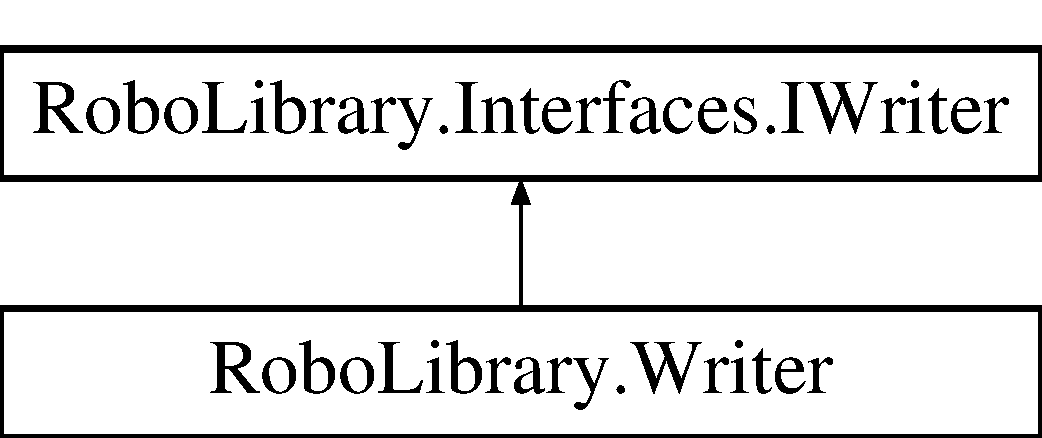
\includegraphics[height=2.000000cm]{class_robo_library_1_1_writer}
\end{center}
\end{figure}
\subsection*{Public Member Functions}
\begin{DoxyCompactItemize}
\item 
\hypertarget{class_robo_library_1_1_writer_a3d530a563c96008ad6803535a0e72b66}{}\label{class_robo_library_1_1_writer_a3d530a563c96008ad6803535a0e72b66} 
{\bfseries Writer} (string ip\+\_\+address)
\item 
\hypertarget{class_robo_library_1_1_writer_aa60ea945142f96abb069c8c23ca77646}{}\label{class_robo_library_1_1_writer_aa60ea945142f96abb069c8c23ca77646} 
void {\bfseries Send\+U\+R\+Pose} (\hyperlink{class_robo_library_1_1_u_r_pose}{U\+R\+Pose} pose)
\item 
\hypertarget{class_robo_library_1_1_writer_a0698c2c9a3b2e75a705aa5e4e04dcc0d}{}\label{class_robo_library_1_1_writer_a0698c2c9a3b2e75a705aa5e4e04dcc0d} 
void {\bfseries Add\+U\+R\+Pose} (\hyperlink{class_robo_library_1_1_u_r_pose}{U\+R\+Pose} pose)
\item 
\hypertarget{class_robo_library_1_1_writer_a9cef38e8b8a8b9395a138f26dfe93817}{}\label{class_robo_library_1_1_writer_a9cef38e8b8a8b9395a138f26dfe93817} 
Configuration\+Data {\bfseries Get\+Configurations} ()
\item 
\hypertarget{class_robo_library_1_1_writer_a2506e4dad74aa2da0bab2377fa1f45e5}{}\label{class_robo_library_1_1_writer_a2506e4dad74aa2da0bab2377fa1f45e5} 
void {\bfseries Send\+Configurations} (Configuration\+Data conf\+Data)
\end{DoxyCompactItemize}


The documentation for this class was generated from the following file\+:\begin{DoxyCompactItemize}
\item 
Robo\+Library/Writer.\+cs\end{DoxyCompactItemize}

%--- End generated contents ---

% Index
\backmatter
\newpage
\phantomsection
\clearemptydoublepage
\addcontentsline{toc}{chapter}{Index}
\printindex

\end{document}
